\documentclass[12pt,a4paper,openright,twoside]{book}
\usepackage[utf8]{inputenc}

\newcommand{\thesislang}{english}
\newcommand{\versionmajor}{0}
\newcommand{\versionminor}{1}
\newcommand{\versionpatch}{2}
\newcommand{\version}{\versionmajor.\versionminor.\versionpatch}
\typeout{Document version: \version}
\usepackage{thesis-style}
\usepackage[utf8]{inputenc}
\usepackage{hyperref}
\usepackage{url}
\usepackage{graphicx}
\usepackage{amssymb}
\usepackage{blkarray}
\usepackage{caption}
\usepackage{subcaption}
\usepackage{biblatex}
\usepackage{amsmath}
\usepackage{algpseudocode}
\usepackage{algorithm}
\usepackage{xcolor}
\usepackage{cleveref}
\usepackage{acronym}
\usepackage{amsfonts}

% \DeclareTextFontCommand{\mytexttt}{\ttfamily\hyphenchar\font=45\relax}


% \usemintedstyle{vs}
\usepackage{svg}
\usepackage[many]{tcolorbox}    	% for COLORED BOXES (tikz and xcolor included)
\addbibresource{bibliography.bib} 
\newtcolorbox{boxK}{
    sharpish corners, % better drop shadow
    boxrule = 0pt,
    toprule = 4.5pt, % top rule weight
    enhanced,
    fuzzy shadow = {0pt}{-2pt}{-0.5pt}{0.5pt}{black!35} % {xshift}{yshift}{offset}{step}{options} 
}

\newcommand{\emailaddr}[1]{\href{mailto:#1}{\texttt{#1}}}
\newcommand*{\scafi}{ScaFi}
\newcommand{\meta}[1]{{\color{blue} #1}}% used for meta-comments
\newcommand{\scarlib}{ScaRLib}
\usepackage{listings}
%!TeX root = paper-2023-coordination-marl-tool.tex
\newcommand\YAMLcolonstyle{\color{red}\mdseries}
\newcommand\YAMLkeystyle{\color{black}\ttfamily}
\newcommand\YAMLvaluestyle{\color{blue}\ttfamily}

\makeatletter

% here is a macro expanding to the name of the language
% (handy if you decide to change it further down the road)
\newcommand\language@yaml{yaml}

\expandafter\expandafter\expandafter\lstdefinelanguage
\expandafter{\language@yaml}
{
  keywords={true,false,null,y,n},
  keywordstyle=\color{darkgray}\bfseries,
  basicstyle=\YAMLkeystyle,                                 % assuming a key comes first
  sensitive=false,
  tabsize=1,
  comment=[l]{\#},
  morecomment=[s]{/*}{*/},
  commentstyle=\color{purple}\ttfamily,
  stringstyle=\YAMLvaluestyle\ttfamily,
  moredelim=[l][\color{orange}]{\&},
  moredelim=[l][\color{magenta}]{*},
  moredelim=**[il][\YAMLcolonstyle{:}\YAMLvaluestyle]{:},   % switch to value style at :
  morestring=[b]',
  morestring=[b]",
  literate={\ \ }{{\ }}1
}

% switch to key style at EOL
\lst@AddToHook{EveryLine}{\ifx\lst@language\language@yaml\YAMLkeystyle\fi}
\makeatother
%!TeX root = paper-2023-coordination-marl-tool.tex

\lstdefinelanguage{scala}{
  keywords={abstract,case,catch,class,def,%
    do,else,extends,false,final,finally,%
    for,if,implicit,import,match,mixin,%
    new,null,object,override,package,%
    private,protected,requires,return,sealed,%
    super,this,throw,trait,true,try,lazy,%
    type,val,var,while,with,yield,forSome},
  otherkeywords={=>,<-,<\%,<:,>:,\#},
  sensitive=true,
  columns=fullflexible,
  morecomment=[l]{//},
  morecomment=[n]{/*}{*/},
  morestring=[b]",
  stringstyle=\ttfamily\color{red!50!brown},
  showstringspaces=false,
  morestring=[b]',
  morestring=[b]""",
  basicstyle=\sffamily\lst@ifdisplaystyle\scriptsize\fi\ttfamily,
  emphstyle=\sffamily\bfseries\ttfamily
}
\definecolor{ddarkgreen}{rgb}{0,0.5,0}
\lstdefinelanguage{scafi}{
  frame=single,
  basewidth=0.5em,
  language={scala},
  keywordstyle=\color{blue}\textbf,
  commentstyle=\color{ddarkgreen},
  keywordstyle=[2]\color{red}\textbf,
  keywords=[2]{rep,nbr,foldhood,foldhoodPlus,aggregate,branch,spawn,mux,mid},
  keywordstyle=[3]\color{gray},
  keywords=[3]{Me,AroundMe,Everywhere,Forever}, %,@@,@@@
  keywordstyle=[4]\color{red}\textbf,
  keywords=[4]{in,out,rd},
  keywordstyle=[5]\color{violet},
  keywords=[5]{evolve,when,andNext,workflow,G,C,broadcast,gossip},
  keywordstyle=[6]\color{orange},
  keywords=[6]{Available,Serving,Done,Waiting,Removing,None,Set}
}

\lstset{language=scafi}
% Please use the
\acrodef{cmarl}[CMARL]{Cooperative Many Agent Reinforcement Learning}
\acrodef{marl}[MARL]{Multi Agent Reinforcement Learning}
\acrodef{dsl}[DSL]{Domain Specific Language}
\acrodef{rl}[RL]{Reinforcement Learning}
\acrodef{vmas}[VMAS]{Vectorized Multi Agent Simulator}
\acrodef{mdp}[MDP]{Markov Decision Process}

\begin{document}

\frontmatter

% ! TeX root = thesis-main.tex
\title{ScaRLib: integrating VMAS for GPU accelerated simulations}
\author{Filippo Cavallari}
\date{\today}

\newgeometry{margin=0.8in}
\begin{titlepage}
	\begin{center}
		% \vspace*{0.2cm}
		
		\large
		\textbf{ALMA MATER STUDIORUM -- UNIVERSITÀ DI BOLOGNA \\ CAMPUS DI CESENA}
		\\
		\noindent\hrulefill
		\vspace{0.4cm}
		
		\Large
		Scuola di Ingegneria e Architettura \\
		Corso di Laurea Magistrale in Ingegneria e Scienze Informatiche
		
		\Huge
		\vspace{4cm}
		\textbf{
			ScaRLib: integrating VMAS for 
			\\
			GPU accelerated simulations
		}
		
		\large
		\vspace{1cm}
		Tesi di laurea in 
		\\
		\textsc{Pervasive Computing}
		
		\vspace{5.5cm}
		\begin{minipage}[t]{0.64\textwidth}
			\begin{flushleft}
				\textit{Relatore} 
				\\ 
				\textbf{Prof.} $\mid$ \textbf{Ing.} $\mid$ \textbf{Dott.} \textbf{Mirko Viroli}, \textbf{PhD}
				\\
				\vspace{0.4cm}
				\textit{Correlatori} 
				\\
				\textbf{Dott.} \textbf{Gianluca Aguzzi}
				\\
				\textbf{Dott.} \textbf{Davide Domini}
			\end{flushleft}
		\end{minipage}
		\begin{minipage}[t]{0.34\textwidth}
			\begin{flushright}
				\textit{Candidato} 
				\\ 
				\textbf{Filippo Cavallari}
			\end{flushright}
		\end{minipage}\\
		
		\vfill
		\noindent\hrulefill
		\vspace{0.3cm}
		\Large
		
		Quarta Sessione di Laurea
		\\
		Anno Accademico 2022-2023
	\end{center}
\end{titlepage}
\restoregeometry

\newpage

\begin{abstract}
This thesis expands ScaRLib, a research Scala framework crafted to facilitate the development of \ac{cmarl} systems that seamlessly integrates learning processes powered by PyTorch.
The framework prioritizes ease of use and powerful system specification by employing numerous abstractions that capture high-level aspects of the \ac{cmarl} domain, abstracting away low-level implementation details.
\ac{vmas} stands as a sophisticated framework tailored for \ac{marl} applications.
Uniquely combining vectorization and 2D physics simulation within the PyTorch framework, \ac{vmas} distinguishes itself through its user-friendly and modular interface. This design facilitates the creation of new scenarios, encouraging community contributions and collaborative development.
The primary objective of this thesis is to integrate \ac{vmas} into ScaRLib, positioning it as a simulation engine concealed behind ScaRLib APIs. 
By achieving this integration, this thesis aims to create a comprehensive tool that combines the high-level specification capabilities of ScaRLib with the sophisticated simulation features of \ac{vmas}. 
The validation of this integration involves the simulation of diverse \ac{cmarl} scenarios, demonstrating the effectiveness and versatility of the unified framework. 
In the end, this work will allow the execution of extremely complex simulations there were not possible before on ScaRLib.
\end{abstract}

% \begin{dedication} % this is optional
%     Optional. Max a few lines.
% \end{dedication}

% \begin{acknowledgements} % this is optional
%     Optional. Max 1 page.
% \end{acknowledgements}

\tableofcontents
\listoffigures
% \lstlistoflistings

\mainmatter

\chapter{\introductionname}
\label{chap:introduction}

The study of \acf{cmarl} has gained considerable attention due to its applicability in tackling complex problems involving multiple intelligent agents. One of the significant challenges in this field is devising and implementing robust algorithms capable of navigating dynamic and unpredictable scenarios. To address this challenge, this thesis introduces the integration of two researchframeworks — ScaRLib and \ac{vmas}.
 
\emph{The goal of this thesis centers on the seamless integration of \ac{vmas}} \cite{bettini2022vmas}, renowned for its unique application of vectorization and 2D physics simulation within the \emph{PyTorch} framework \cite{paszke2019pytorch}, \emph{into ScaRLib}, a user-friendly Scala framework for high-level specifications. \emph{This integration aims to harness the PyTorch-powered simulation capabilities of \ac{vmas}}, through ScaRLib's API, \emph{effectively bringing together the simplicity of ScaRLib} alongside the sophistication of \ac{vmas} in a unified toolkit for \ac{cmarl}.

Once the integration is complete, we plan to showcase the versatility and efficacy of this unified platform by simulating a variety of \ac{cmarl} scenarios. This demonstration is intended to show the potential applicability of the newly integrated framework within the broader \ac{cmarl} field.

The ultimate aim here is not to revolutionize the domain of \ac{cmarl}, but rather to provide a valuable tool to the community of researchers and practitioners. By giving researchers access to a platform that combines high-level specification capabilities with advanced simulation features, we hope to support continued advancements in the field of \ac{cmarl}, easing the path to exploring and executing complex tasks requiring multiple intelligent agents.
\newpage
\section{Structure of the Thesis}

The remainder of this thesis is organized as follows:
\begin{enumerate}
    \item \textbf{\Cref{chap:background} - Background:} Provides an overview of \ac{marl}, Deep Q-Learning, ScaRLib, and \ac{vmas}, laying the foundation for the subsequent chapters.
    \item \textbf{\Cref{chap:analysis} - Analysis:} Describes the ubiquitous language used in the project and lists its functional and technical requirements.
    \item \textbf{\Cref{chap:implementation} - Implementation:} Details the implementation of the \ac{vmas} module within the ScaRLib framework, focusing on actions, states, environment, rendering, logging, and the \ac{dsl}.
    \item \textbf{\Cref{chap:validation} - Validation:} Presents a perfomance comparison between Alchemist and \ac{vmas} and a usage showcase of the unified framework through a specific scenario—Cleaning Agents. This chapter outlines perfomance gap between the two simulators, as well as the objectives, reward functions, implementation details, and results of the implemented \ac{cmarl} scenario.
    \item \textbf{\Cref{chap:conclusion} - Conclusion:} Recaps the aims, methodologies, and findings of the thesis, reflecting primarily on the effective application of the VMAS module within the ScaRLib framework for MARL systems. This chapter discusses the potential for wider adoption of these advancements across academia and the industrial sector while also acknowledging the limitations and possible focal points for future exploration. The conclusion serves to subtly affirm the significance of the thesis and its contribution to the evolving landscape of MARL systems.
    \item \textbf{Bibliography:} Lists the references and sources used throughout the thesis.
\end{enumerate}

\chapter{Background} % or Background
\label{chap:background}

\section{Reinforcement Learning and Deep Q-Learning}

\subsection{Overview}

Deep Q-Learning (DQL) stands as a groundbreaking stride in \ac{rl}, merging Q-Learning principles with the power of deep neural networks. In this chapter, we will delve into the fundamental aspects of DQL, exploring its core concepts, the algorithms it relies on, the Bellman equation, and its practical applications \cite{DBLP:journals/corr/MnihKSGAWR13}.

\subsection{Reinforcement Learning}

The history of \ac{rl} is deeply intertwined with the development of AI and Machine Learning. 
Early work in \ac{rl} was influenced primarily by research in psychology during the mid-twentieth century. The term \emph{reinforcement} is 
derived from learning theories of B.F. Skinner and other behavioural psychologists. Richard Sutton and Andrew Barto later 
formalized these ideas into the RL framework in their book ``\emph{Reinforcement Learning: An Introduction}'' \cite{Sutton1998}. 
Despite these early developments, it was not until the recent decades, coupled with advanced computational power and storage 
capabilities, that \ac{rl} gained significant attraction.

Nowadays, \ac{rl} stands as a subcategory of machine learning where an agent learns to make decisions by interacting with an environment. 
Unlike other types of machine learning where data is given upfront, in \ac{rl}, the agent collects data by exploring the environment.
The primary goal of an agent in reinforcement learning is to maximize some notion of cumulative reward. 
This is achieved through a series of interactions between the agent and the environment. 
In each interaction, the agent decides an action based on the current state of the environment, and the environment, in return, provides a reward and the new state. 
The agent's behavior is determined by its policy - a mapping from the perceived states of the environment to the actions the agent wants to take. 
The agent’s task is to find an optimal policy, which maximizes the expected cumulative reward. The flow of \ac{rl} is summerized in \Cref{fig:j}.

\begin{figure}
    \centering
    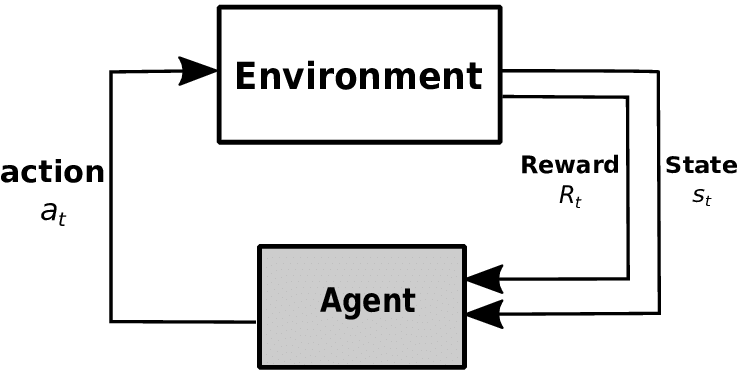
\includegraphics[width=8cm]{img/rl.png}
    \caption{\ac{rl} steps}
    \label{fig:j}
\end{figure}

The prominent mathematical framework that models the above interactions is known as the \ac{mdp}. The \ac{mdp} framework comprises a set of states ($S$), a set of actions ($A$), a reward function ($R$) and a state transition function ($T$). 
The reward function maps each state-action pair to a real number, signifying the expected immediate reward after performing an action in a state. 
The state transition function specifies the probabilities of moving from one state to another after taking an action.

\ac{rl} can be subdivided into different types as illustrated in \Cref{fig:z}:
\begin{figure}
    \centering
    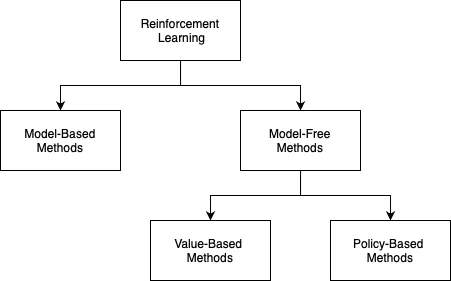
\includegraphics[width=8cm]{img/typesofrl.jpg}
    \caption{Types of \ac{rl}}
    \label{fig:z}
\end{figure}
\begin{enumerate}
    \item \textbf{Model-based RL:} in model-based \ac{rl} \cite{DBLP:journals/corr/abs-2006-16712}, \emph{the agent learns} or has a model of \emph{the environment} which it utilizes to make decisions on what actions to take.
    \item \textbf{Model-free RL:} differing from model-based \ac{rl}, in model-free \ac{rl} \cite{Sutton1998}, \emph{the agent} has no explicit model of the environment and must \emph{learn to make decisions based on experiences}. Both Q-learning \cite{qlearning} and \emph{Deep Q-Learning} fall into this category.
    \item \textbf{Value-based RL vs Policy-based RL:} in value-based \ac{rl} \cite{Sutton1998}, the agent primarily learns a value function, with the optimal policy derived from this value function. In contrast, policy-based \ac{rl} directly learns the optimal policy without having to learn a value function \cite{inbook}.
    \item \textbf{On-policy vs Off-policy RL:} on-policy learning \cite{andrychowicz2020matters} involves learning the value of a policy while following it. Off-policy learning \cite{degris2013offpolicy} involves learning the value of a policy while following another policy. \emph{Q-learning} is an example of off-policy as it learns the optimal policy while following an exploration policy.
\end{enumerate}

It has been also applied across a wide range of domains (\Cref{fig:y}):
\begin{figure}
    \centering
    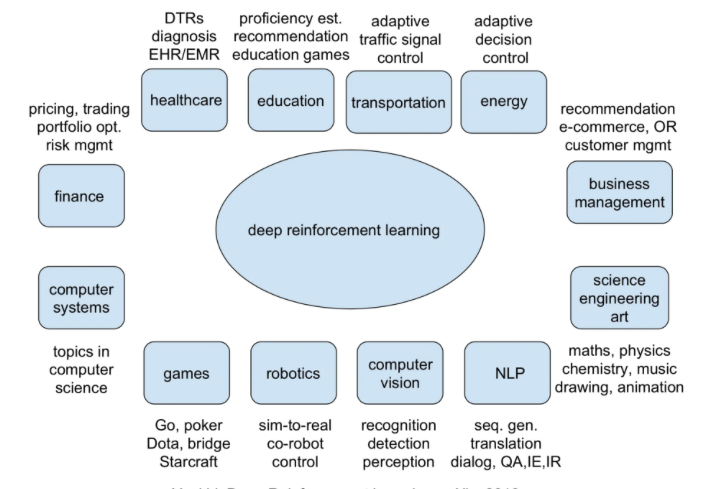
\includegraphics[width=8cm]{img/applicationsofrl.png}
    \caption{Applications of \ac{rl}}
    \label{fig:y}
\end{figure}
\begin{enumerate}
    \item \textbf{Robotics:} \ac{rl} is extensively used to train robots for various tasks \cite{robotics2030122}. It could be teaching a four-legged robot to walk or a robotic hand to manipulate objects independently.
    \item \textbf{Autonomous Vehicles:} \ac{rl} can be used to optimize the path planning, control, and decision-making systems of self-driving cars \cite{MARTINEZDIAZ2018275}.
    \item \textbf{Natural Language Processing:} \ac{rl} can optimize tasks that require sequential decision making in NLP \cite{nlp-rl}, such as dialogue systems and machine translation.
    \item \textbf{Finance:} \ac{rl} agents can learn investment and trading strategies, portfolio management, and risk management \cite{finance-rl}.
\end{enumerate}

At the heart of \ac{rl} algorithms lies \emph{Q-Learning} (\Cref{fig:k}) \cite{qlearning}, a 
formative method that constructs an action-value function, commonly denoted 
as $Q(s, a)$. The action-value function, or \emph{Q-function}, quantifies the expected 
cumulative reward that an agent can anticipate receiving, assuming it takes a 
specific action ($a$) in a given state ($s$ ) and thereafter follows an optimal policy.

An optimal policy refers to the strategy that, if followed, would lead to the 
maximum cumulative reward from any given state. The principle behind determining 
such a policy is rooted in the Bellman Equation. According to it, the value of a state under an 
optimal policy is equal to the maximum expected value attainable by taking an 
action and then continuing optimally from the resulting state. This equation (\Cref{eq:q_learning})
provides a recursive definition of the optimal policy.

\begin{equation}
    Q(s, a) = r + \gamma \max_{a'} Q(s', a')
    \label{eq:q_learning}
\end{equation}

Where:
\begin{align*}
    Q(s, a) & \text{ is the Q-value of state } s \text{ and action } a. \\
    r & \text{ is the immediate reward for taking action } a \text{ in state } s. \\
    \gamma & \text{ is the discount factor determining the importance of future rewards.} \\
    s' & \text{ is the next state resulting from taking action } a \text{ in state } s. \\
    \max_{a'} Q(s', a') & \text{ represents the maximum Q-value achievable in the next state } s' \\
    & \text{ considering all possible actions } a'.
\end{align*}

Q-Learning employs an iterative update rule to continually refine the Q-values 
until they converge towards the optimal values implied by the Bellman Equation. 
The update rule is based on adjusting the agent's estimated returns according to 
the difference between its predicted reward and the 
reward actually received after taking an action.

This mechanism of constantly updating and improving Q-values continues until the 
predictions made by the Q-Function match the actual rewards obtained, which is 
when the Q-values have ``converged''. This convergence indicates that the agent's 
predictions and the Bellman optimal values have become consistent, thus leading 
to the development of the optimal policy.

A critical dilemma in \ac{rl} is the trade-off between exploration and exploitation. 
In the $\varepsilon$-Greedy strategy, the agent usually exploits the environment by selecting the action with the highest Q-value. However, occasionally with an $\varepsilon$ probability, it chooses a random action, thereby ensuring exploration of the environment.

But there are other methods to perform exploration, including:
\begin{enumerate}
    \item \textbf{Softmax Exploration \cite{softmax-exploration}:} here the policy is often based on the Boltzmann distribution. The action-selection is more informed - actions with higher reward probability are more likely to be picked.
    \item \textbf{Upper Confidence Bound \cite{10.5555/944919.944941}:} here the greediness is tempered by the measure of uncertainty or the lack of confidence about the action's outcomes.
    \item \textbf{Noisy Nets \cite{fortunato2019noisy}:} artificial noise is added to the weights of the network, encouraging the agent to explore the environment.
\end{enumerate}
Each method has its innate advantages and disadvantages - the effectiveness depends on the task at hand. 

\subsection{Deep Q-Learning}

In DQL, a deep neural network is used to approximate the \emph{Q-function} (\Cref{fig:k}). A deep neural network typically consists of an input layer, one or more hidden layers, and an output layer. The input layer represents the state of the environment. The output layer, on the other hand, represents the \emph{Q-value} for each possible action. The hidden layers, usually fully connected and containing a significant number of nodes, enable the network to learn complex, non-linear relationships.
This network takes the current state $s$ as input and outputs a \emph{Q-value} for each possible action $a$. The agent selects the action with the highest \emph{Q-value}, guiding its decision-making process.
\begin{figure}
    \centering
    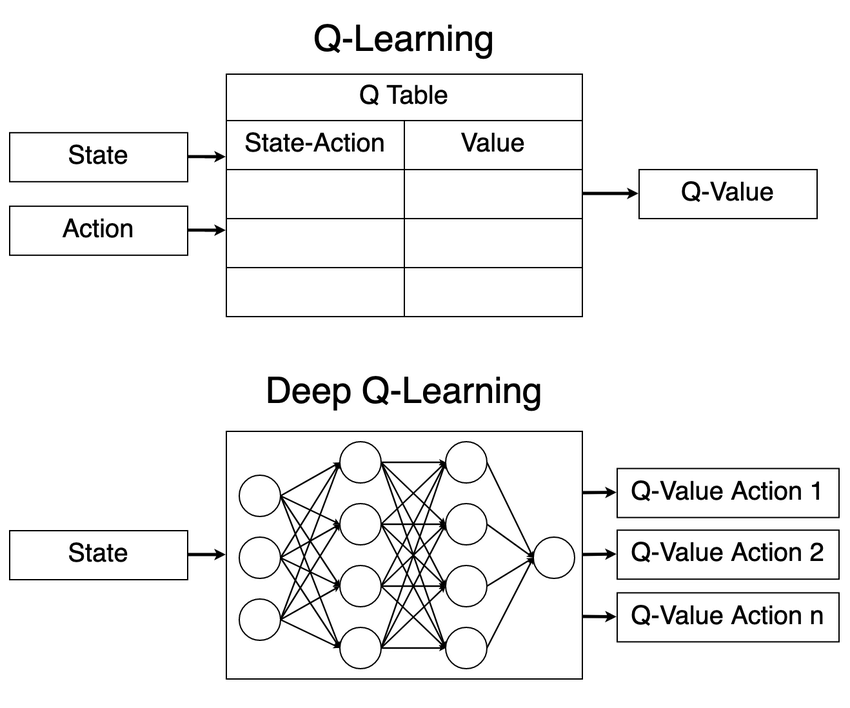
\includegraphics[width=8cm]{img/dql.png}
    \caption{Q-learning and Deep Q-learning architecture}
    \label{fig:k}
\end{figure}

Training a deep neural network involves feeding the network a set of inputs (states of the environment, in this case) and adjusting the weights and biases in the network using a process called backpropagation.

As expected, an appropriate loss functions has to be used to measure the difference between the \emph{predicted Q-value} and \emph{the real (or target) Q-value}; such function is called \emph{Q-Loss} and is updated using the Bellman equation. 

The final goal of training the network is to minimize this loss: by observing the gradient of the loss function with respect to the network parameters allows us to perform an update in the direction of steepest descent, often modified by a learning rate. 

Optimization algorithms such as \emph{stochastic gradient descent (SGD)} or more advanced versions such as \emph{Adam} or \emph{RMSprop} are often used. The choice of optimizer can have a significant impact on the speed and stability of learning.


The Q-learning loss is typically calculated as follows:
\[
L(\theta) = \mathbb{E}\left[(Q(s, a;\theta) - (r + \gamma \max_{a'}Q(s', a';\theta^-))^2\right]
\]
where:
\begin{align*}
L(\theta) & \text{ is the loss with respect to the network's parameters }\theta. \\
Q(s, a;\theta) & \text{ is the predicted Q-value for state }s\text{ and action }a\text{ with network parameters }\theta. \\
r & \text{ is the immediate reward received after taking action }a\text{ in state }s. \\
\gamma & \text{ is the discount factor that determines the importance of future rewards.} \\
s' & \text{ is the next state after taking action }a\text{ in state }s. \\
\theta^- & \text{ are the parameters of the target Q-network.}
\end{align*}

In sequential tasks such as reinforcement learning, the action taken at a given step is heavily influenced by the preceding state. This sequential dependency can lead to strong correlations between consecutive samples. When the agent subsequently trains on these correlated samples, this results in a twisting of the data that the agent learns from, thereby establishing a narrow, biased learning and leading to overfitting. Overfitting in this context means that the agent performs exceptionally well in the learned situations, but fails to generalize to new ones.

Let us consider an agent trained to play a racing game-like environment. If it only learns from a sequence of highly correlated states where the task is to avoid an obstacle on the right, it may overfit its policy to always steer left, even in situations when it is not optimal.

To mitigate this, a technique often used in Deep Q Learning is the introduction of a replay buffer. The replay buffer stores a history of state transitions, allowing the agent to sample experiences randomly during training. This random sampling helps to break these potentially harmful correlations, providing a more diverse learning experience for the agent and promoting a more robust policy that can generalize better to unseen situations.

By storing the agent's experiences at each time-step during its interaction with the environment, and using this stored information for learning later, the replay buffer allows us to recycle this experience data, making the learning algorithm also more data-efficient.

The use of a \emph{separate target network} is a crucial component in \emph{stabilizing the learning process}. The parameters of the target network are copied from the main \emph{Q-network} every $T$ timesteps, where $T$ is a hyperparameter we select. 

The idea is to provide stable target values during the learning process: without the target network, we would be moving our targets at every learning step and that can lead to divergence or oscillation of the learning process. 

\subsubsection{DQL Algorithm}

The core DQL algorithm can be summarized in several steps, described in \Cref{dql-algorithm}.

\begin{algorithm}[H]
    \caption{Deep Q-Learning Algorithm}\label{dql-algorithm}
    \begin{algorithmic}[1]
        \State Initialize the Q-network and the target network with random weights
        \State Initialize the replay buffer
        \For{each episode}
            \State Observe the current state $s$
            \State Select an action $a$ using epsilon-greedy policy
            \State Execute action $a$, observe reward $r$ and next state $s'$
            \State Store the experience $(s, a, r, s')$ in the replay buffer
            \State Sample a mini-batch from the replay buffer
            \State Calculate the target Q-values using the target network
            \State Calculate the loss between predicted and target Q-values using the Bellman equation
            \State Update the Q-network weights using backpropagation
            \State Periodically update the target network weights
        \EndFor
    \end{algorithmic}
\end{algorithm}

\subsubsection{Challenges, improvements and applications}

Despite its success, DQL encounters challenges that researchers actively address for further refinement. Training instability, stemming from non-smooth and non-stationary environments, poses a hurdle. Additionally, \emph{Q-value} overestimation, where the algorithm tends to overestimate the expected cumulative rewards, can affect performance. Moreover, the demand for extensive data collection raises concerns about efficiency.

To mitigate these challenges, researchers have introduced innovative improvements:

\begin{enumerate}
    \item \textbf{Double DQN \cite{vanhasselt2015deep}:} this enhancement aims to reduce overestimation by decoupling the action selection from the action evaluation, leading to more accurate Q-value estimates.
    \item \textbf{Prioritized Experience Replay \cite{schaul2016prioritized}:} by assigning different priorities to experiences in the replay buffer based on their learning potential, this technique prioritizes more informative samples during the training process.
    \item \textbf{Dueling DQN \cite{wang2016dueling}:} this modification separates the estimation of the value function and the advantage function, enabling the network to better understand the value of each action.
\end{enumerate}
These advancements contribute to the robustness and efficiency of DQL in various applications.

Deep Q-Learning has found successful applications across diverse domains, showcasing its versatility and adaptability:

\begin{enumerate}
\item \textbf{Atari Games}: DQL has demonstrated human-level performance on various Atari 2600 games \cite{mnih2013playing}, showcasing its ability to learn intricate strategies and excel in complex gaming environments.
\item \textbf{Robotics}: in the field of robotics \cite{quillen2018deep}, DQL is instrumental in training robots for tasks such as object manipulation, navigation, and control, contributing to advancements in autonomous systems.
\item \textbf{Autonomous Vehicles}: DQL plays a crucial role in training autonomous vehicles \cite{liu2023comparative}, enhancing their ability to navigate safely and efficiently in dynamic and unpredictable environments.
\item \textbf{Recommendation Systems}: online platforms leverage DQL to optimize recommendation systems \cite{CHEN2023110335}, providing users with personalized and relevant content based on their preferences and behaviors.
\item \textbf{Healthcare}: in healthcare, DQL is applied to optimize treatment plans and resource allocation \cite{MUNDRU202339}, contributing to the efficient management and delivery of healthcare services.
\end{enumerate}

These applications underscore the broad impact and potential of Deep Q-Learning in addressing complex challenges across various industries.
    
\newpage

\section{MARL}

\subsection{Overview}
A multi-agent system comprises multiple entities that, with a certain degree of independence, make decisions 
and interact with each other within an environment \cite{weiss1999multiagent}. Each agent is assigned a task to pursue, which can be 
either the same as others (\emph{cooperative}) or different (\emph{competitive}). To address a specific task, an agent 
requires a set of skills. Expressing these competencies programmatically would be particularly complex. Hence, the decision was made to employ \ac{rl}, 
giving rise to the term \emph{Multi-Agent Reinforcement Learning}, for which the following definition can be provided:

\emph{``A group of agents collectively learns the best policy to maximize a long-term reward function.''}

\subsection{Environment}
These two characteristics introduce complexities compared to \emph{Single-Agent Reinforcement 
Learning (SARL)}. In SARL, the learning process is modeled as a \emph{Markov Decision Process (MDP)},
 which is inherently stationary by definition. Consequently, SARL inherently assumes a single
  agent engaged in the learning process, with the remaining agents considered as part of the 
  environment.

In the case of \ac{marl}, \ac{rl} is integrated using an additional abstraction 
known as \emph{Stochastic Game S (or Markov Games)} \cite{LITTMAN1994157}:

\begin{itemize}
  \item $\mathcal{S}$ is a tuple $<N, S, \{A^i\}, P,  \{R^i\}>$ with $i \in 1..N$
  \item N is the number of agents (must be greaten than 1 but has no upper-bound)
  \item S is always a space of values that represent the global state of the system
  \item $A^i$ is the action space of the i-th agent
  \begin{itemize}
       \item The global space is defined as $\mathbb{A} = A^1 \times A^2 \times .... \times A^N$
  \end{itemize}
  \item $P: S \times \mathbb{A} \rightarrow \mathcal{P}(S)$ is the function that describes the steps between each state
  \begin{itemize}
      \item $P(S)$ is discrete probability distribution that pairs each state $s \in S$ with a probability
  \end{itemize}
  \item $R^i: S \times \mathbb{A} \times S \rightarrow \mathbb{R}$ is the reward function
\end{itemize}

\begin{boxK}
\textbf{\textit{Example of Markov Game: Paper, Rock and Scissor}}

  \begin{itemize}
    \item $N = 2$
    \item $A^1 = A^2 = $ \{Paper, Rock, Scissor\}
    \item $S = $ \{ \}
    \item $R = \begin{blockarray}{cccc}
      & Rock & Paper & Scissor \\
    \begin{block}{c[ccc]}
      Rock    & 0, 0  & -1, 1 & 1, -1 \\
      Paper   & 1, -1 & 0, 0  & -1, 1 \\
      Scissor & -1, 1 & 1, -1 & 0, 0 \\
    \end{block}
  \end{blockarray}$
  \end{itemize}
\end{boxK}

\subsubsection{Types of MARL}
\ac{marl} systems can be categorized in various ways, and one primary division is as follows \cite{4445757}:

% \begin{figure}
%     \centering
%     \includesvg[width=11cm]{img/MARL-Divisione1.svg}
% \end{figure}

\begin{itemize}
    \item \textbf{\textit{Cooperative}}: in cooperative \ac{marl}, all agents within the system share the same goal, and consequently, the same reward function $(R^1 = ... = R^i = ... = R^N)$.
    \begin{itemize}
        \item \textbf{\textit{Homogeneous}}: in homogeneous cooperative \ac{marl}, all agents have identical capabilities $(A^1 = ... = A^i = ... = A^N)$; the overall objective is to find the best policy. % which is usually the same for each agent $(\pi^* = \pi^*_1 = ... = \pi^*_N)$.
        \item \textbf{\textit{Heterogeneous}}: in heterogeneous cooperative \ac{marl}, agents may possess varying capabilities, and in the worst-case scenario, each agent has different capabilities from all others $(A^1 \neq ... \neq A^i \neq ... \neq A^N)$. The global objective is to maximize each agent's local policy while pursuing the shared goal.
    \end{itemize}
    \item \textbf{\textit{Competitive}}: competitive \ac{marl} involves agents with different goals who compete to maximize their own reward functions. A typical example of such systems is board games.
    \item \textbf{\textit{Mixed}}: in mixed \ac{marl}, both cooperative agents with a shared goal and competitive agents with different goals coexist. A classic example is team-based games where players on the same team cooperate while players from different teams compete.
\end{itemize}

Further division can be made based on how the training and execution of various agents occur:

% \begin{figure}
%     \centering
%     \includesvg[width=11cm]{img/MARL-Divisione2.svg}
% \end{figure}

\begin{itemize}
    \begin{figure}
    \centering
    \includegraphics[width=8cm]{img/CTCE.png}
    \caption{CTCE System \cite{aguzzi}}
    \label{fig:a}
    \end{figure}

    \item \textbf{\textit{Centralized Training Centralized Execution}} (\Cref{fig:a}): In this type of system, a higher-level ``Learner'' agent with a global perspective is responsible for training and computing actions. The remaining agents send their local environment perceptions (local states) to the Learner agent, who reconstructs the global state. The Learner agent then selects actions according to the current policy, evaluates reward functions, and updates the policy (learning process). This approach is typically used for offline training of the system.
    
    \begin{figure}
    \centering
    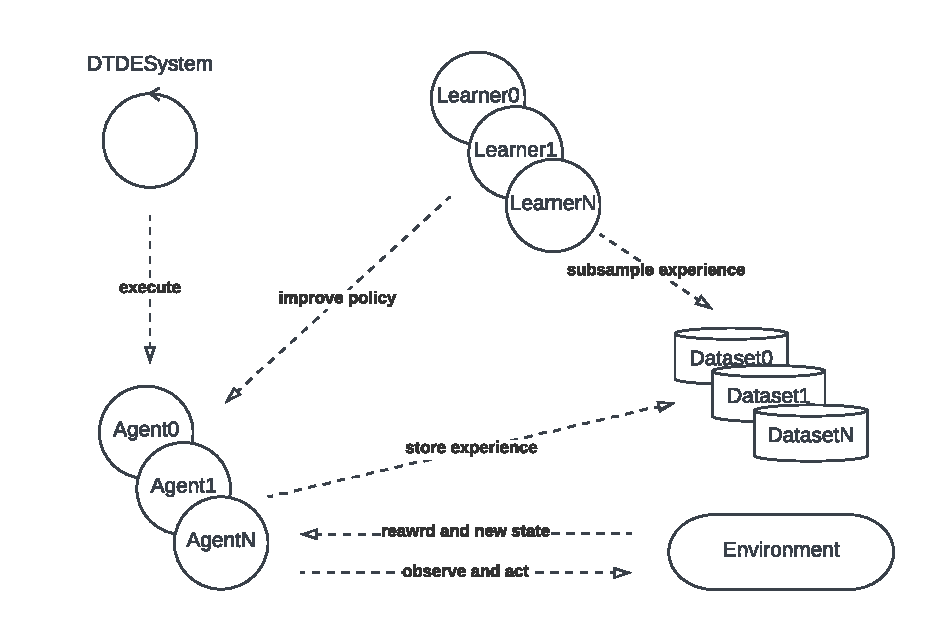
\includegraphics[width=8cm]{img/DTDE.png}
    \caption{DTDE System \cite{aguzzi}}
    \label{fig:b}
    \end{figure}

    \item \textbf{\textit{Decentralized Training Decentralized Execution}} (\Cref{fig:b}): In this type of system, each agent has its local policy and can only perceive a portion of the environment. Each agent takes actions based on its perception of the environment, updating its local reward function accordingly. This approach is used for both offline training and online deployment of the system.
    
    \begin{figure}
      \centering
      \includegraphics[width=8cm]{img/CTDE.png}
      \caption{CTDE System \cite{aguzzi}}
      \label{fig:c}
      \end{figure}
    
    \item \textbf{\textit{Centralized Training Decentralized Execution}} (\Cref{fig:c}): In this type of system, two distinct steps are involved:
    \begin{enumerate}
        \item \textbf{\textit{Simulation Time}}: Each agent uses its local policy, and at the end of each episode, they send their respective information to a central Learner agent. This Learner agent, with a global view of the environment, updates the local policies of the various agents.
        \item \textbf{\textit{Execution Time}}: During this phase, each agent uses its local policy (resulting from the training process) to interact with the environment.
    \end{enumerate}
    
\end{itemize}

\newpage

\section{ScaRLib}
ScaRLib \footnote{The tool is available on GitHub at \url{https://github.com/ScaRLib-group/ScaRLib}}
\footnote{A demo video is accessible at: \url{https://github.com/ScaRLib-group/ScaRLib-demo-video}} is an 
innovative Scala framework tailored for advancing the development of \ac{cmarl} systems through JVM-based high-level specification. 
The learning process is seamlessly executed under the hood using \emph{PyTorch}\footnote{\url{https://pytorch.org/}}.

This project's primary objective is to furnish a tool that facilitates both straightforward and robust system specification. 
To achieve this, we have crafted numerous abstractions that capture high-level aspects of the \ac{marl} domain, abstracting away the intricacies of low-level 
implementation details.

Essentially, \scarlib{} comprises three principal modules (\Cref{fig:modules}):
\begin{enumerate}
    \item \texttt{scarlib-core}, responsible for implementing the main abstractions over the \ac{cmarl} domain;
    \item \texttt{dsl-core}, which offers a high-level language for specifying the system;
    \item \texttt{alchemist-scafi}, establishing bindings between \scarlib{} and the Alchemist and \scafi{} tools.
\end{enumerate}

It is essential to note that while \scarlib{} currently includes the Alchemist-Scafi combination module to address existing needs, 
it is not restricted to this combination alone. The framework is flexible enough to support the implementation of other bindings to diverse tools. 
For instance, one can replace Alchemist with an alternative simulator such as FLAME GPU~\cite{flame} or, as this thesis shows, \ac{vmas}~\cite{bettini2022vmas}.

\begin{figure}[t]
    \centering
    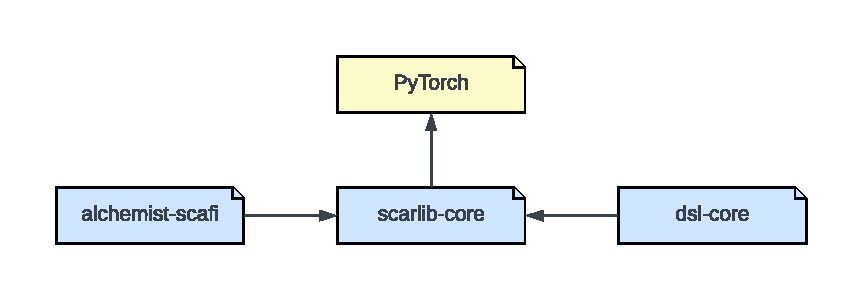
\includegraphics[width=0.7\textwidth]{img/scarlib-modules.pdf}
    \caption{ScaRLib main modules \cite{scarlib}}
    \label{fig:modules}
\end{figure}

\paragraph{Core Abstraction:} The \texttt{scarlib-core} module serves as the foundational component, implementing core functionalities and abstractions within the framework. This includes the definition of essential data structures and the implementation of key algorithms (\Cref{fig:arc}).

All abstractions (\Cref{fig:arc}) revolve around fundamental concepts, with the central element being the \texttt{System}. This entity comprises agents interacting within a shared environment, trained to optimize a global or local reward signal expressed by a reward function.

Two pre-implemented system types, widely recognized in literature~\cite{Du2020}, are provided: i) centralized training and decentralized execution (\texttt{CTDESystem}), and ii) decentralized training and execution (\texttt{DTDESystem}). Additionally, the framework incorporates an implementation of the DQN algorithm~\cite{Mnih2015}, used for agent training.

To define a custom system with a specific collective goal, end-users need only implement four elements: i) the environment, ii) the agent state space, iii) the action space, and iv) the reward function. Utilizing this module alone enables the execution of a learning process in a simulated environment based on the platform.

\begin{figure}[t]
    \centering
    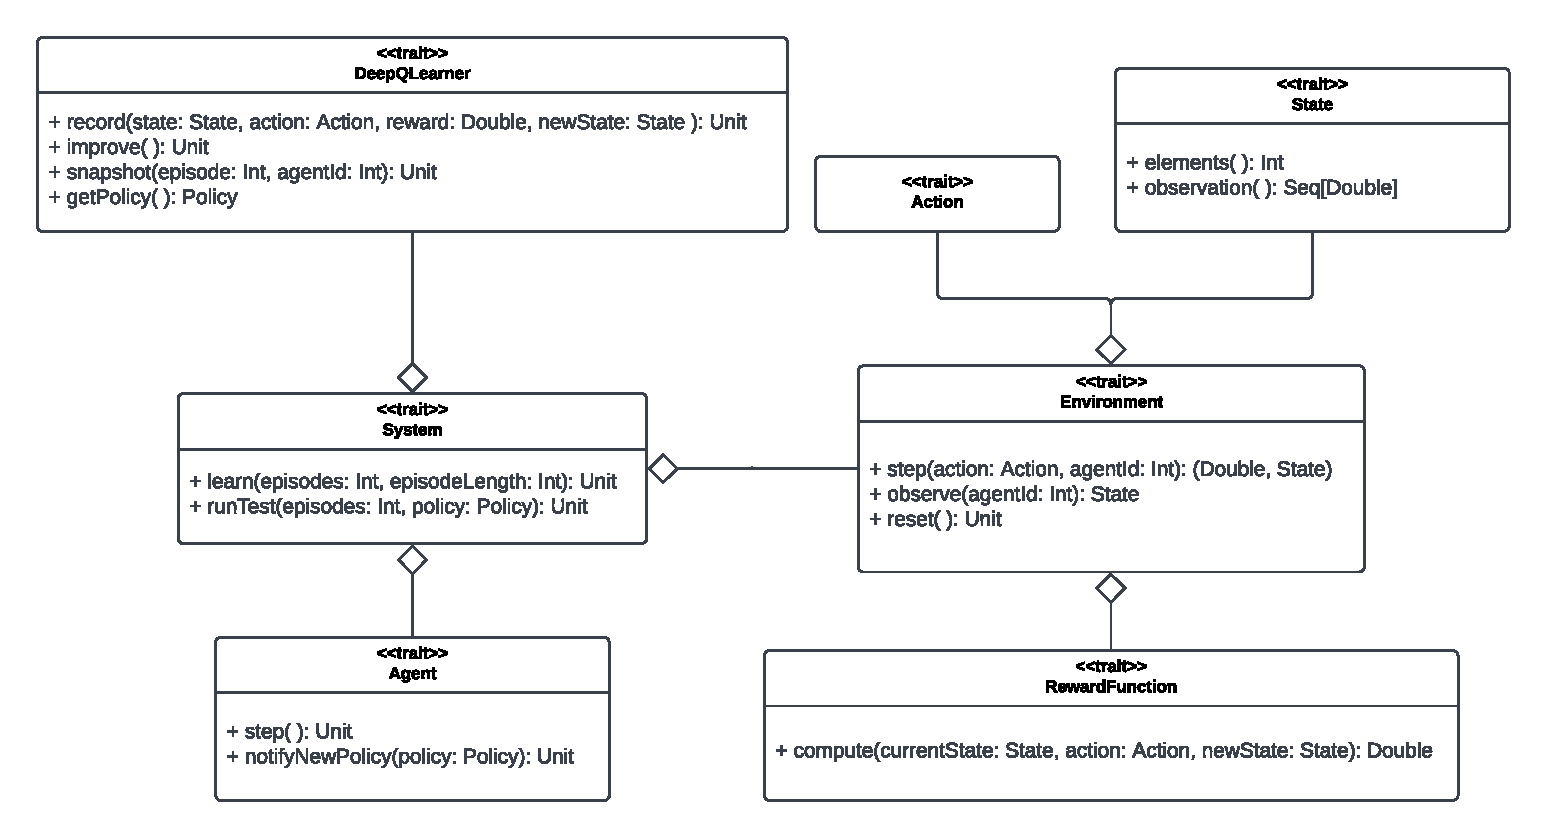
\includegraphics[width=\textwidth]{img/core-architecture.pdf}
    \caption{\scarlib{} Core Architecture \cite{scarlib}}
    \label{fig:arc}
\end{figure}

To comprehend the system dynamics, it is beneficial to delve into the internals. Both systems employ a training process organized into multiple \emph{epochs}, each containing a set of \emph{episodes}. Agents receive the current state as input during an episode, execute an action, and collectively drive the environment to the next state. At an epoch's end, the environment resets, and agents are trained using the accumulated experience.

For a \texttt{CTDESystem} (\Cref{fig:ctde}), agents are trained centrally, sharing global experience in a single central dataset. A central learner oversees the training process and enhances the policy neural network. The system is also responsible for agent execution and policy update notifications, allowing easy extension for concurrent and distributed execution.

The \texttt{DTDESystem} (\Cref{fig:dtde}) operates similarly, but each agent possesses its dataset and learner.

Regarding the training process, \scarlib{} supports neural-network-based \ac{rl} algorithms (e.g., DQN) and utilizes PyTorch, the current standard for building neural networks. The integration with PyTorch is facilitated through ScalaPy \cite{Laddad2020}, allowing direct interaction with PyTorch and its associated libraries.

Integration typically involves setting up a Python environment with instantiated libraries and creating a Scala API isolating necessary interactions with the Python ecosystem. In \scarlib{}, this is achieved through DQN, serving as the entry point for accessing Torch.

\begin{figure*}[t]
    \centering
    \begin{subfigure}[b]{0.49\textwidth}
        \centering
        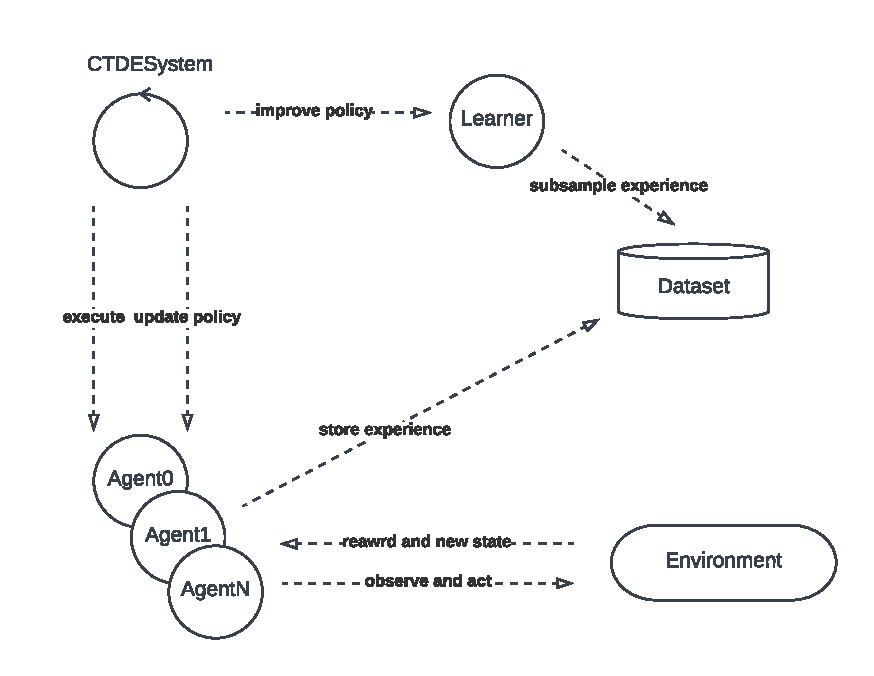
\includegraphics[width=\textwidth]{img/ctdesystem.pdf}
        \caption{CTDE System \cite{scarlib}}
        \label{fig:ctde}
    \end{subfigure}
    \begin{subfigure}[b]{0.49\textwidth}
        \centering
        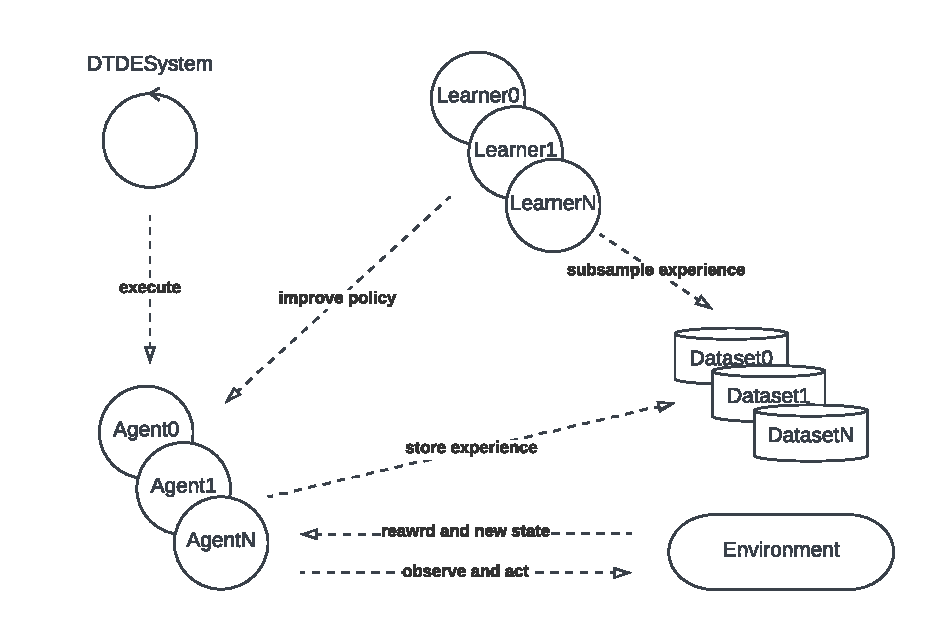
\includegraphics[width=\textwidth]{img/DTDE.pdf}
        \caption{DTDE System \cite{scarlib}}
        \label{fig:dtde}
    \end{subfigure}
\caption{Examples of Developed System Dynamics. On the left, a centralized system with a global learner updating a shared policy. On the right, a decentralized system where each agent has a local policy and learner.}
\end{figure*}

\paragraph{ScaFi-Alchemist Integration:} In addition to the core functionality, we have introduced the \texttt{alchemist-scafi} module (\Cref{fig:alchemist-arc}), facilitating integration with the tools Alchemist \cite{DBLP:journals/jos/PianiniMV13} and \scafi{} \cite{Casadei2022}. This integration empowers the execution of the learning process within an aggregate computing context, a crucial aspect of our contribution. Previous \ac{cmarl} applications with Alchemist and ScaFi suffered from ad-hoc solutions, lacking reusability, flexibility, and interoperability between Alchemist and chosen native libraries \cite{DBLP:conf/acsos/AguzziCV22}. Our integration aims to provide a comprehensive and reusable system, bridging the gap between the Many-agent RL community and the Alchemist simulator within this paradigm.

The specification of a learning system remains unchanged, with only two new elements introduced: the definition of the Alchemist simulation and the implementation of the \scafi{}-based logic.

To define an Alchemist simulation (\Cref{fig:alchemist}), a \scafi{} class is passed as a program to the \texttt{AlchemistEnvironment}. This class contains aggregate programming code defining the simulation dynamics. The training process advances through the injection of a molecule containing the current action (a subtype of the \texttt{Action} class) by a learner that incorporates the \ac{rl} policy. The aggregate program evaluates the environment state (a subtype of \texttt{State}) using \texttt{computeState} and inserts it into the \texttt{state} molecule, utilized by the learner for policy updates.

\begin{figure}[t]
    \centering
    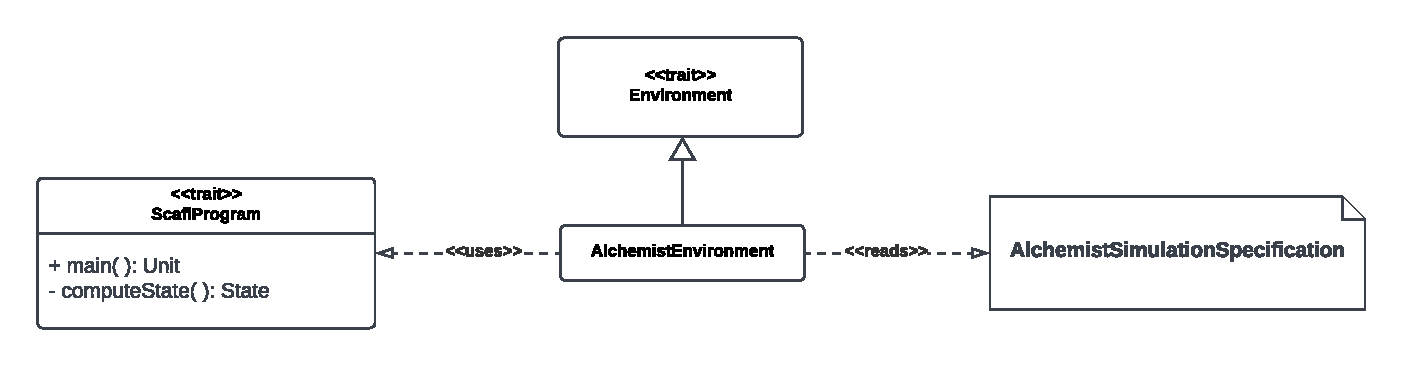
\includegraphics[width=\textwidth]{img/alchemist-scafi-arc.pdf}
    \caption{\scarlib{} \texttt{alchemist-scafi} architecture. A \texttt{ScafiProgram} should be passed to the \texttt{AlchemistEnvironment} to initiate the learning process.}
    \label{fig:alchemist-arc}
\end{figure}

\begin{figure*}
    \centering
    \begin{subfigure}[b]{0.49\textwidth}
        \centering
        \begin{lstlisting}[language=yaml]
incarnation: scafi
network-model:
    type: ConnectWithinDistance
    parameters: [0.5]
deployments:
    type: Grid
    parameters: [-5,-5,5,5,0.25,0.25]
    /*dynamics of the simulation*/
    programs: 
        - program:
        - time-distribution: 1
            type: Event
            actions: 
            - type: RunScafiProgram
              parameters: [program]
        - program: send
        \end{lstlisting}
    \end{subfigure}
    \hfill
    \begin{subfigure}[b]{0.49\textwidth}
        \centering
        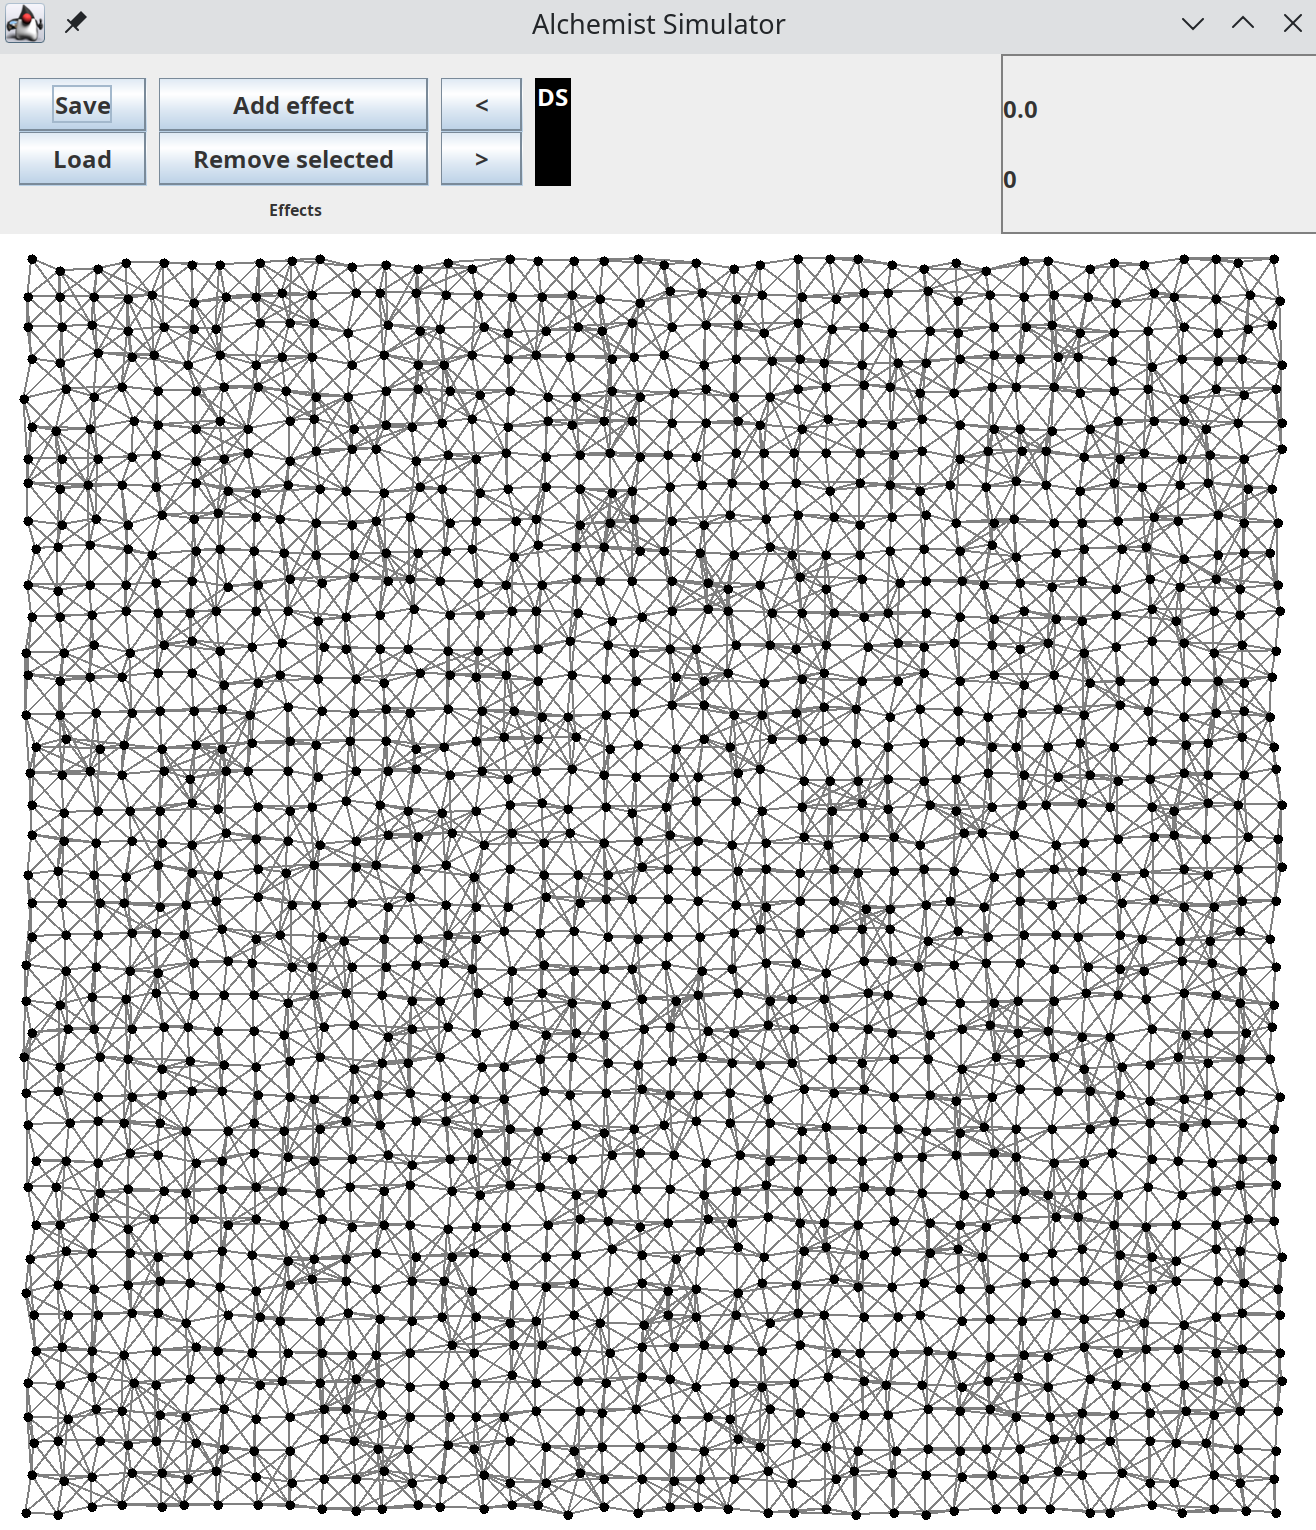
\includegraphics[width=\textwidth]{img/alchemist.png}
    \end{subfigure}
    \caption{An Alchemist simulation example. The simulation result on the right is obtained by running the simulation described on the left.}
    \label{fig:alchemist}
\end{figure*}

\paragraph{DSL for Learning Configurations:} The most recent module introduced is an internal DSL designed for the agile and flexible creation of \ac{cmarl} training systems. This choice aims to bridge the gap between the \ac{marl} system designer's conceptualization and the realization of the training system. Leveraging a language like Scala for the DSL enables the capture of errors during compilation, providing early feedback on configuration issues before actual system runs.

The presented DSL serves as a straightforward facade to the abstractions featured in the \texttt{scarlib-core} module. Consequently, to initiate a simulation (e.g., in Alchemist), developers need to define a reward function indicating how favorable the current state of a particular agent is relative to the environmental condition:
\begin{lstlisting}
  class MyRewardFunction extends CollectiveRewardFunction:
      override def computeReward(state: State, action: Action, nextState: State): Double = ...
  \end{lstlisting}
  Subsequently, developers must specify the actions supported by agents within the chosen system. Assuming an identical action space for each agent in \ac{cmarl} systems, actions can be defined as a product type:
  \begin{lstlisting}
    sealed trait MyAction extends Action
    object MyAction:
        case object A extends MyAction
        case object B extends MyAction
        case object C extends MyAction
        def all: Seq[MyAction] = Seq(A, B, C)
    \end{lstlisting}
    Final configurations involve selecting the class of the Alchemist environment to instantiate, defining the number of agents, and specifying the buffer size for storing memory:
    \begin{lstlisting}
      val system = learningSystem {
          rewardFunction { new MyRewardFunction() }
          actions { MyAction.all}
          dataset { ReplayBuffer[State, Action](10000) }
          agents { 50 } // select the number of agent
          environment {
              // select a specific environment
              "it.unibo.scarlib.experiments.myEnvironment"
          }
      }
      \end{lstlisting}
\section{Vectorized Multi-Agent Simulator (VMAS)}

\subsection{Introduction to VMAS}

\ac{vmas} is a unique framework designed for efficient \ac{marl} simulations \cite{bettini2022vmas}. It consists of a vectorized 2D physics engine implemented in PyTorch and a set of challenging multi-robot scenarios. The platform's modular design encourages easy scenario creation and contributions from the community. \ac{vmas} simulates agents and landmarks with different shapes, supporting rotations, elastic collisions, joints, and custom gravity. Holonomic motion models simplify agent simulation, and custom sensors like \emph{LiDARs} are available. The vectorization in PyTorch enables \ac{vmas} to perform simulations in batches, scaling seamlessly to tens of thousands of parallel environments on accelerated hardware.

\subsection{Performance and GPU Acceleration}

The key differentiator of \ac{vmas} lies in its combination of multi-agent learning and environment vectorization. Vectorization is crucial for accelerating \ac{marl} training, where on-policy iterations involve simulated team rollouts and policy updates. \ac{vmas}'s vectorization allows parallel simulation, significantly reducing the time needed for collecting rollouts. In comparison to OpenAI MPE, \ac{vmas} demonstrates remarkable speed-ups. While MPE's execution time increases linearly with the number of simulations, \ac{vmas} can execute 30,000 parallel simulations in under 10 seconds, proving more than 100 times faster. The platform leverages GPU acceleration to achieve these impressive results.

\subsection{Structure and Design Principles}

\ac{vmas} is structured to adhere to several design principles.

\begin{enumerate}
    \item Vectorized: \ac{vmas}'s vectorization capability allows it to step any number of environments in parallel, crucial for efficient \ac{marl} training.
    \item Simple: While complex vectorized physics engines exist, \ac{vmas} uses a simple custom 2D dynamics engine written in \emph{PyTorch}, ensuring fast simulation without sacrificing computational speed.
    \item General: \ac{vmas} is designed to support various high-level multi-robot problems in 2D, accommodating both adversarial and cooperative scenarios. It employs holonomic robot simulation, focusing on high-level coordination without the need to learn low-level controls using \ac{marl}.
    \item Extensible: \ac{vmas} is not just a simulator but a framework that enables the creation of new multi-agent scenarios. Its modular structure facilitates new task creation, and interactive rendering aids scenario debugging.
    \item Compatible: \ac{vmas} provides compatibility with different \ac{marl} interfaces, including RLlib and Gym, offering seamless integration with a range of RL algorithms.
\end{enumerate}


\subsection{VMAS Architecture}
\begin{figure}[t]
    \centering
    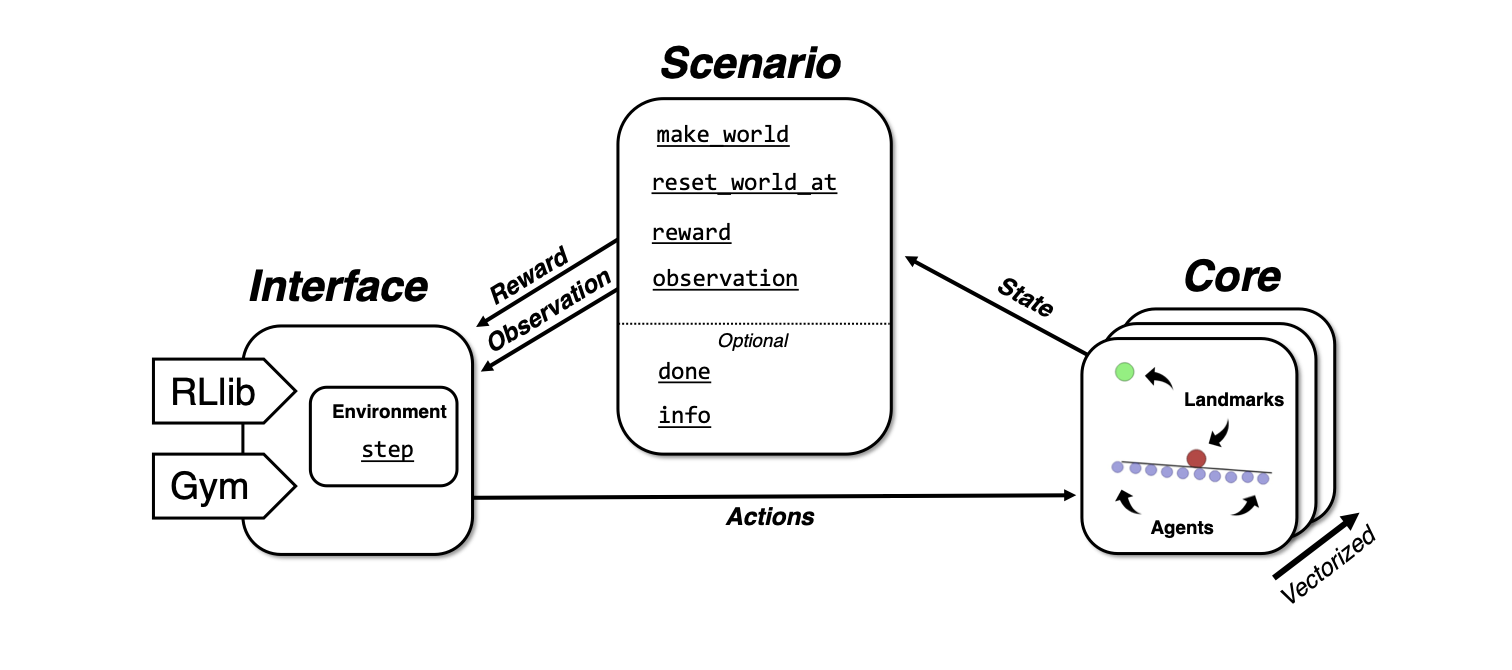
\includegraphics[width=\textwidth]{img/vmasstructure.png}
    \caption{\ac{vmas} architecture}
    \label{fig:v}
\end{figure}
The structure of \ac{vmas} is divided into three main components: \emph{Interface}, \emph{Scenario}, and \emph{Core} (\Cref{fig:v}).

\subsubsection{Interface}
\ac{vmas} has a vectorized interface that allows stepping any number of environments in parallel. It supports \emph{PyTorch} for feeding tensors directly as input/output. Additionally, \ac{vmas} provides wrappers for the non-vectorized OpenAI Gym interface and the vectorized interface of the RLlib framework. The interface enables rendering through Pyglet.

\subsubsection{Scenario}
Scenarios in \ac{vmas} encode multi-agent tasks that the team aims to solve. Custom scenarios can be implemented with ease, taking advantage of interactive rendering for quick debugging. Scenarios define functions like make\_world (creating agents and landmarks), reset\_world\_at (resetting environments), reward (calculating rewards), and observation (returning agent observations).

\subsubsection{Core}
The core of \ac{vmas} is where the world simulation takes place. It contains entities, representing agents and landmarks, and a 2D physics module written in \emph{PyTorch}. The simulation step involves basic 2D dynamics using a force-based physics engine, allowing holonomic motion for entities.

\subsection{Physics Simulation in VMAS}

\ac{vmas}'s physics engine utilizes a force-based approach with a semi-implicit Euler method for integrating the state. It includes collision simulation, gravity, and torque calculations. Entities in the world have shapes (sphere, box, or line) and vectorized states containing position, velocity, rotation, and angular velocity. The simulation step handles both linear and angular states, providing a comprehensive physics simulation for 2D multi-agent scenarios.

\subsection{Multi-robor scenarios and comparison with MPE}
\begin{figure}[t]
    \centering
    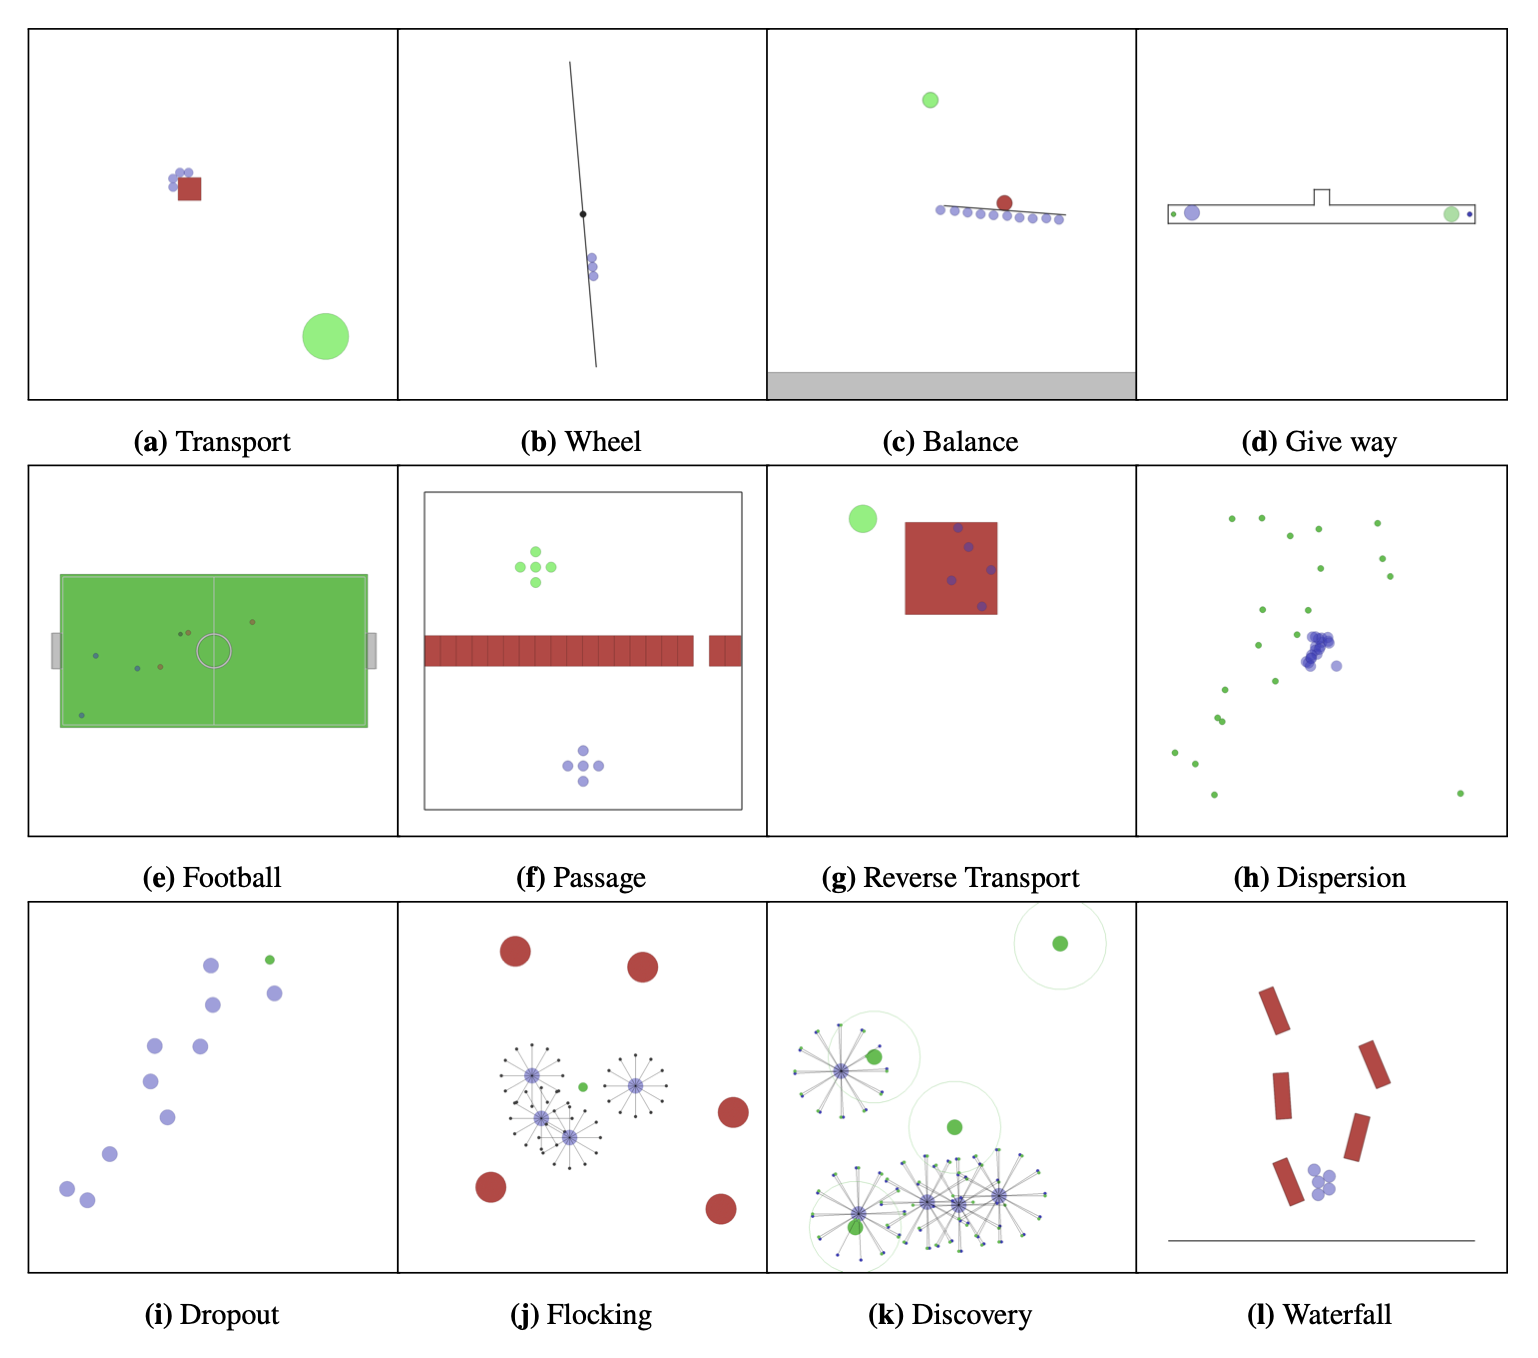
\includegraphics[width=\textwidth]{img/vmasscenarios.png}
    \caption{Scenarios introduced by \ac{vmas}}
    \label{fig:u}
\end{figure}
The \ac{vmas} researchers have introduced 12 multi-robot scenarios alongside the framework (\Cref{fig:u}), all of which requires complex coordination like leveraging heterogeneous behavior and inter-agent communication to solve. These scenarios delimit the agents' input by defining the set of their observations, such as position, velocity, sensory input, and goal position all can be modified to increase or decrease the difficulty of the scenario.

The tasks within these scenarios can be customized and each scenario comes with a local heuristic test set. Additionally, they have ported all 9 scenarios from MPE (Multi-Policy Environment \cite{lowe2020multiagent}) to \ac{vmas}.

The new scenarios include tasks such as transporting a package, rotating a line, balancing a line, giving way to another agent, playing football, passing through a barrier, reverse transport, dispersion, reaching a goal, flocking around a target, quick coverage of targets, and moving through a series of obstacles.
\begin{figure}[t]
    \centering
    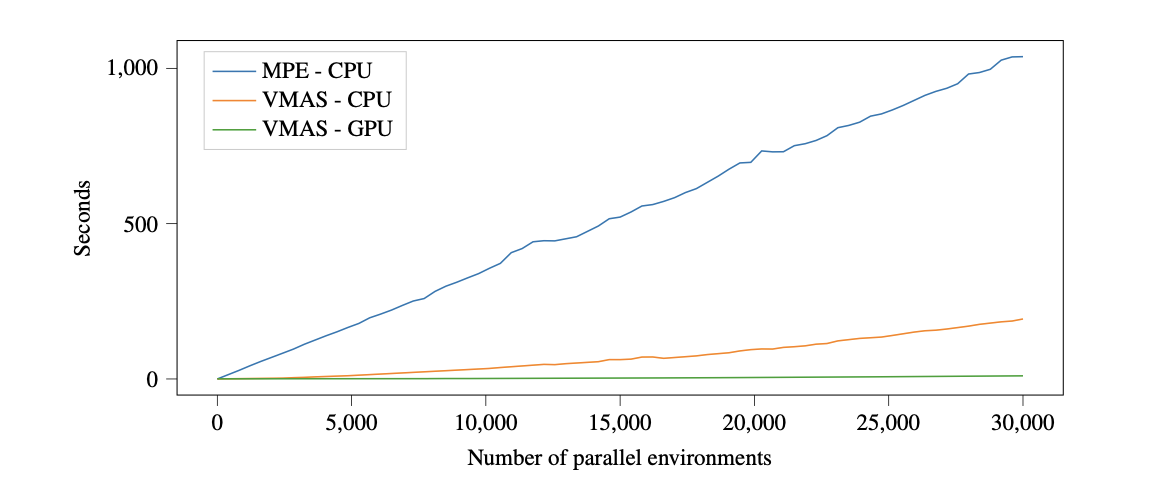
\includegraphics[width=\textwidth]{img/vmasvsmpe.png}
    \caption{Perfomance comparison of \ac{vmas} and MPE}
    \label{fig:t}
\end{figure}
The comparison between VMAS and MPE (\Cref{fig:t}) shows the impact of vectorization on simulation speed, with VMAS achieving up to 5x faster execution time on CPU and up to 100x faster on GPU.

\begin{figure}[t]
    \centering
    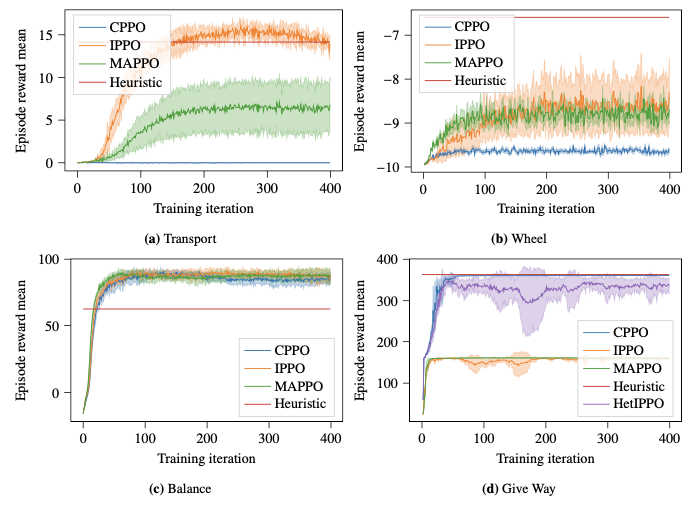
\includegraphics[width=\textwidth]{img/vmas4scen.png}
    \caption{Benchmarking of four different \ac{rl} algorithms on VMAS scenarios}
    \label{fig:s}
\end{figure}
The researchers also conducted training experiments to benchmark the performance of \ac{marl} algorithms on four \ac{vmas} scenarios (\Cref{fig:s}). The models compared were all based on Proximal Policy Optimization, an actor-critic \ac{rl} algorithm. The models comparison include CPPO (centralized critic and actor), MAPPO (centralized critic and decentralized actor), IPPO (decentralized critic and actor) and HetIPPO (no parameter sharing, each agent’s model is unique).

The results showcase VMAS capabilities in providing a challenging environment for developing sophisticated MARL algorithms, indicating that no single solution can fit all the challenges presented in these scenarios. Lastly, vectorization streamlining the learning process, which is critical for the wider adoption of multi-agent learning in the robotics community.

\subsection{Conclusion}

In conclusion, \ac{vmas} stands as an open-source platform for efficient \ac{marl} simulations, leveraging \emph{PyTorch}'s vectorization capabilities. Its performance benefits from GPU acceleration, allowing parallel simulations at an unprecedented scale. The platform's design principles of being simple, general, extensible, and compatible make it a valuable tool for the \ac{marl} community. \ac{vmas} demonstrates its prowess by challenging state-of-the-art \ac{marl} algorithms with its scenarios, proving difficult in orthogonal ways. Future plans include extending features, implementing new scenarios, and modularizing the physics engine for increased flexibility.

\newpage

\chapter{Analysis}
\label{chap:analysis}

\section{Ubiquitous Language}

In the realm of \ac{cmarl}, a well-defined and shared language is paramount for effective communication among developers, researchers, and users. This chapter delves into the key terminologies forming the backbone of the integrated ScaRLib-VMAS framework, providing a comprehensive guide to the ubiquitous language.

\subsection{Key Concepts in MARL}

\textbf{Agents:}\\
\textit{Definition:} Autonomous entities within the simulation, capable of making decisions and taking actions.\\
\textit{Significance:} Agents are the fundamental actors in the \ac{cmarl} environment, embodying autonomous decision-makers.\\

\textbf{Environment:}\\
\textit{Definition:} The virtual world in which agents operate, providing the context for their interactions and learning.\\
\textit{Significance:} The environment sets the stage for agent interactions, influencing learning and decision-making processes.\\

\textbf{Deep Q-Learning:}\\
\textit{Definition:} A machine learning technique used for training agents through a deep neural network to approximate Q-values, guiding decision-making.\\
\textit{Significance:} Deep Q-Learning is a foundational technique for training intelligent agents, influencing their policy through Q-value approximation.\\

\textbf{Replay Buffer:}\\
\textit{Definition:} A memory device used in reinforcement learning and in particular in Deep Q-Learning, storing state, action, reward, and next state transitions.\\
\textit{Significance:} Replay buffer improves the learning of an agent by breaking harmful correlations through random sampling and by making it more data-efficient.\\

\textbf{Bellman Equation:}\\
\textit{Definition:} Mathematical formulation used in Deep Q-Learning for Q-value approximation, influencing the agent's optimal policy.\\
\textit{Significance:} The Bellman Equation guides the learning process by formulating the relationship between current and future Q-values.\\

\textbf{Policy:}\\
\textit{Definition:} Strategy or rule that an agent follows to determine the next action based on the current state.\\
\textit{Significance:} A policy determines the behavior of an agent in an environment and optimizing a policy can maximize an agent's cumulative reward.\\

\textbf{Reward:}\\
\textit{Definition:} Immediate feedback received by an agent for the action taken in a specific state.\\
\textit{Significance:} It determines the learning objective of an agent and steers its policy in reinforcement learning.\\

\subsection{ScaRLib Terminology}

\textbf{DSL (Domain Specific Language):}\\
\textit{Definition:} High-level language for specifying \ac{cmarl} scenarios within ScaRLib, abstracting away implementation details.\\
\textit{Significance:} DSL simplifies the specification of scenarios, allowing users to focus on high-level concepts without delving into low-level intricacies.\\

\textbf{Actions and States:}\\
\textit{Definition:} Essential components defining the agent's decision space and the observable aspects of the environment.\\
\textit{Significance:} Actions and states form the core of an agent's interaction with the environment, shaping the decision-making process.\\

\textbf{Rendering and Logging:}\\
\textit{Definition:} Processes within ScaRLib responsible for visualizing the simulation and recording relevant data for analysis.\\
\textit{Significance:} Rendering and logging facilitate the analysis and understanding of the simulated scenarios, aiding in debugging and evaluation.\\

\textbf{Alchemist:}\\
\textit{Definition:} A discrete event simulator (DES), where each simulation event is executed one at a time, advancing the simulation's overall timeline accordingly. This approach allows for easy modeling of events placed in time with a variety of temporal distributions.\\
\textit{Significance:} Alchemist is flexible and able to simulate a wide range of phenomena, from chemical reactions to pedestrian movements, as long as these phenomena can be expressed in terms of Alchemist's model. This model comprises distinct abstract entities, whose specifics depend on the particular category of simulations, or in other words, their specific incarnation. The terminology used in Alchemist is derived from chemistry due to its origin from purely chemical models.\\

\subsection{VMAS Components}

\textbf{Vectorized Multi-Agent Simulator:}\\
\textit{Definition:} A sophisticated framework combining vectorization and 2D physics simulation within \emph{PyTorch}, designed for \ac{marl} applications.\\
\textit{Significance:} \ac{vmas} provides a powerful platform for efficient \ac{marl} benchmarking, leveraging \emph{PyTorch}'s capabilities for vectorized simulations.\\

\textbf{Python:}\\
\textit{Definition:} An interpreted, high-level, general-purpose programming language.\\
\textit{Significance:} Python is widely used in fields like data science, machine learning and web development for its simplicity and clarity of syntax. It is the programming language used to write \ac{vmas}.\\

\textbf{Thread:}\\
\textit{Definition:} The smallest sequence of programmed instructions that can perform a task independently.\\
\textit{Significance:} Threads enable concurrent programming for efficient execution of complex programs.\\

\textbf{Tensor:}\\
\textit{Definition:} A mathematical object that generalizes scalars, vectors, and higher-order matrices.\\
\textit{Significance:} Tensors allow the processing of complex multi-dimensional data sets, crucial for many machine learning applications.\\

\textbf{Observation Function:}\\
\textit{Definition:} A function which maps the state of a VMAS scenario's environment to the agent's observation in the form of a tensor.\\
\textit{Significance:} It helps define the agent’s understanding or perception of the environment's state and forms the basis of the agent's decision-making procedure.\\

\textbf{Reward Function:}\\
\textit{Definition:} A function in a VMAS scenario that provides feedback or reward to an agent for every action it takes.\\
\textit{Significance:} The reward function guides the agent to learn the best policy for achieving the maximum cumulative reward.\\

\textbf{Performance and GPU Acceleration:}\\
\textit{Definition:} \ac{vmas}'s capabilities for efficient simulation, leveraging GPU's computational power for enhanced performance.\\
\textit{Significance:} GPU acceleration enables \ac{vmas} to achieve remarkable speed-ups, optimizing computational efficiency in parallel simulations.\\

\textbf{Scenario Creation:}\\
\textit{Definition:} The process of generating new scenarios within \ac{vmas}, encouraging collaborative development and community contributions.\\
\textit{Significance:} Scenario creation allows for the exploration of diverse and challenging environments, fostering community collaboration and innovation.\\

\subsection{Unified Framework}

\textbf{Objective:}\\
\textit{Definition:} The overarching goal of seamlessly integrating \ac{vmas} into ScaRLib, creating a unified framework for \ac{cmarl} simulations.\\
\textit{Significance:} The unified framework aims to provide a cohesive and versatile environment for \ac{cmarl} simulations, simplifying the development and experimentation process.\\

\textbf{High-level Specification:}\\
\textit{Definition:} Leveraging the JVM for high-level specification capabilities, abstracting low-level details for ease of use.\\
\textit{Significance:} High-level specification enhances the accessibility and usability of the framework, allowing users to focus on scenario design rather than implementation intricacies.\\

\textbf{Validation:}\\
\textit{Definition:} Demonstrating the effectiveness and versatility of the integrated framework through diverse \ac{cmarl} scenarios.\\
\textit{Significance:} Validation ensures that the integrated framework meets the intended goals, providing evidence of its utility across a range of scenarios.\\

\textbf{Benchmarking:}\\
\textit{Definition:} The process of comparing the performance of one's system against a standard or best practices.\\
\textit{Significance:} It provides targets and comparative measures, offering insights for improvements.\\

\textbf{Binding:}\\
\textit{Definition:} A technique used in programming that allows the functionalities of one programming language to be used and accessed from another language.\\
\textit{Significance:} Binding enables programs to take advantage of the strengths and specific features of different languages. In the specific case of the thesis realization, binding was utilized to integrate Python's extensive libraries and machine learning capabilities, in particular VMAS, within the ScaRLib framework.\\

\section{Project Requirements}

The successful integration of \ac{vmas} into the ScaRLib framework aims to meet various functional and technical requirements. This section outlines the key aspects that define the project's success.

\subsection{Functional Requirements}

\subsubsection{FRQ1: Seamless Integration}
The integration should provide a seamless experience for users of the ScaRLib framework. Users should be able to leverage \ac{vmas} functionalities without encountering disruptions in the high-level specification and simulation processes.

\subsubsection{FRQ2: High-Level Specification Capabilities}
The unified framework must retain and enhance the high-level specification capabilities of ScaRLib. Users should continue to benefit from the abstraction of low-level details, enabling easy scenario design and experimentation.

\subsubsection{FRQ3: Versatile Scenario Simulation}
The integrated framework should allow the simulation of a broad range of \ac{cmarl} scenarios. Users should be able to create and simulate diverse scenarios, ranging from cooperative to competitive multi-agent setups.

\subsubsection{FRQ4: Usability and Accessibility}
The framework should prioritize usability and accessibility. Users, including researchers and practitioners, should find it intuitive to work with the integrated system, promoting widespread adoption and experimentation.

\subsubsection{FRQ5: Community Collaboration}
Encouraging collaboration within the community is a functional requirement. The integrated framework should facilitate the creation and sharing of new \ac{cmarl} scenarios, fostering a collaborative environment for continuous development.

\subsection{Technical Requirements}

\subsubsection{TRQ1: API Consistency}
The APIs exposed by the unified framework must maintain consistency with ScaRLib's existing structure. This consistency ensures that users familiar with ScaRLib can seamlessly transition to the integrated system.

\subsubsection{TRQ2: Efficient Simulation Performance}
The integration should not compromise the simulation performance achieved by \ac{vmas}. The framework should leverage \ac{vmas}'s vectorization and \emph{PyTorch} capabilities to efficiently simulate complex scenarios with multiple agents.

\subsubsection{TRQ3: Scalability}
The integrated framework should demonstrate scalability, allowing users to scale simulations to handle larger numbers of agents and more intricate scenarios. This ensures that the framework remains robust as the complexity of \ac{cmarl} experiments increases.

\subsubsection{TRQ4: Documentation}
Comprehensive documentation is a technical requirement. It should cover the integrated framework's functionalities, APIs, and best practices, enabling users to understand and utilize the system effectively.

\subsubsection{TRQ5: Error Handling and Debugging}
The integrated framework should provide robust error handling mechanisms and debugging support. Users should receive meaningful error messages, and debugging tools should aid in identifying issues during scenario development and simulation.

\subsubsection{TRQ6: Compatibility}
The unified framework should maintain compatibility with relevant software dependencies, including Java, Scala, \emph{PyTorch}, and \ac{vmas}. Compatibility ensures a smooth user experience across different environments.

By meeting these functional and technical requirements, the integrated ScaRLib-\ac{vmas} framework aims to provide a powerful and user-friendly environment for the development, experimentation, and collaboration in the field of \ac{cmarl}.

\newpage

\chapter{Implementation} % possible chapter for Projects
\label{chap:implementation}

\section{VMAS module}
\begin{figure}
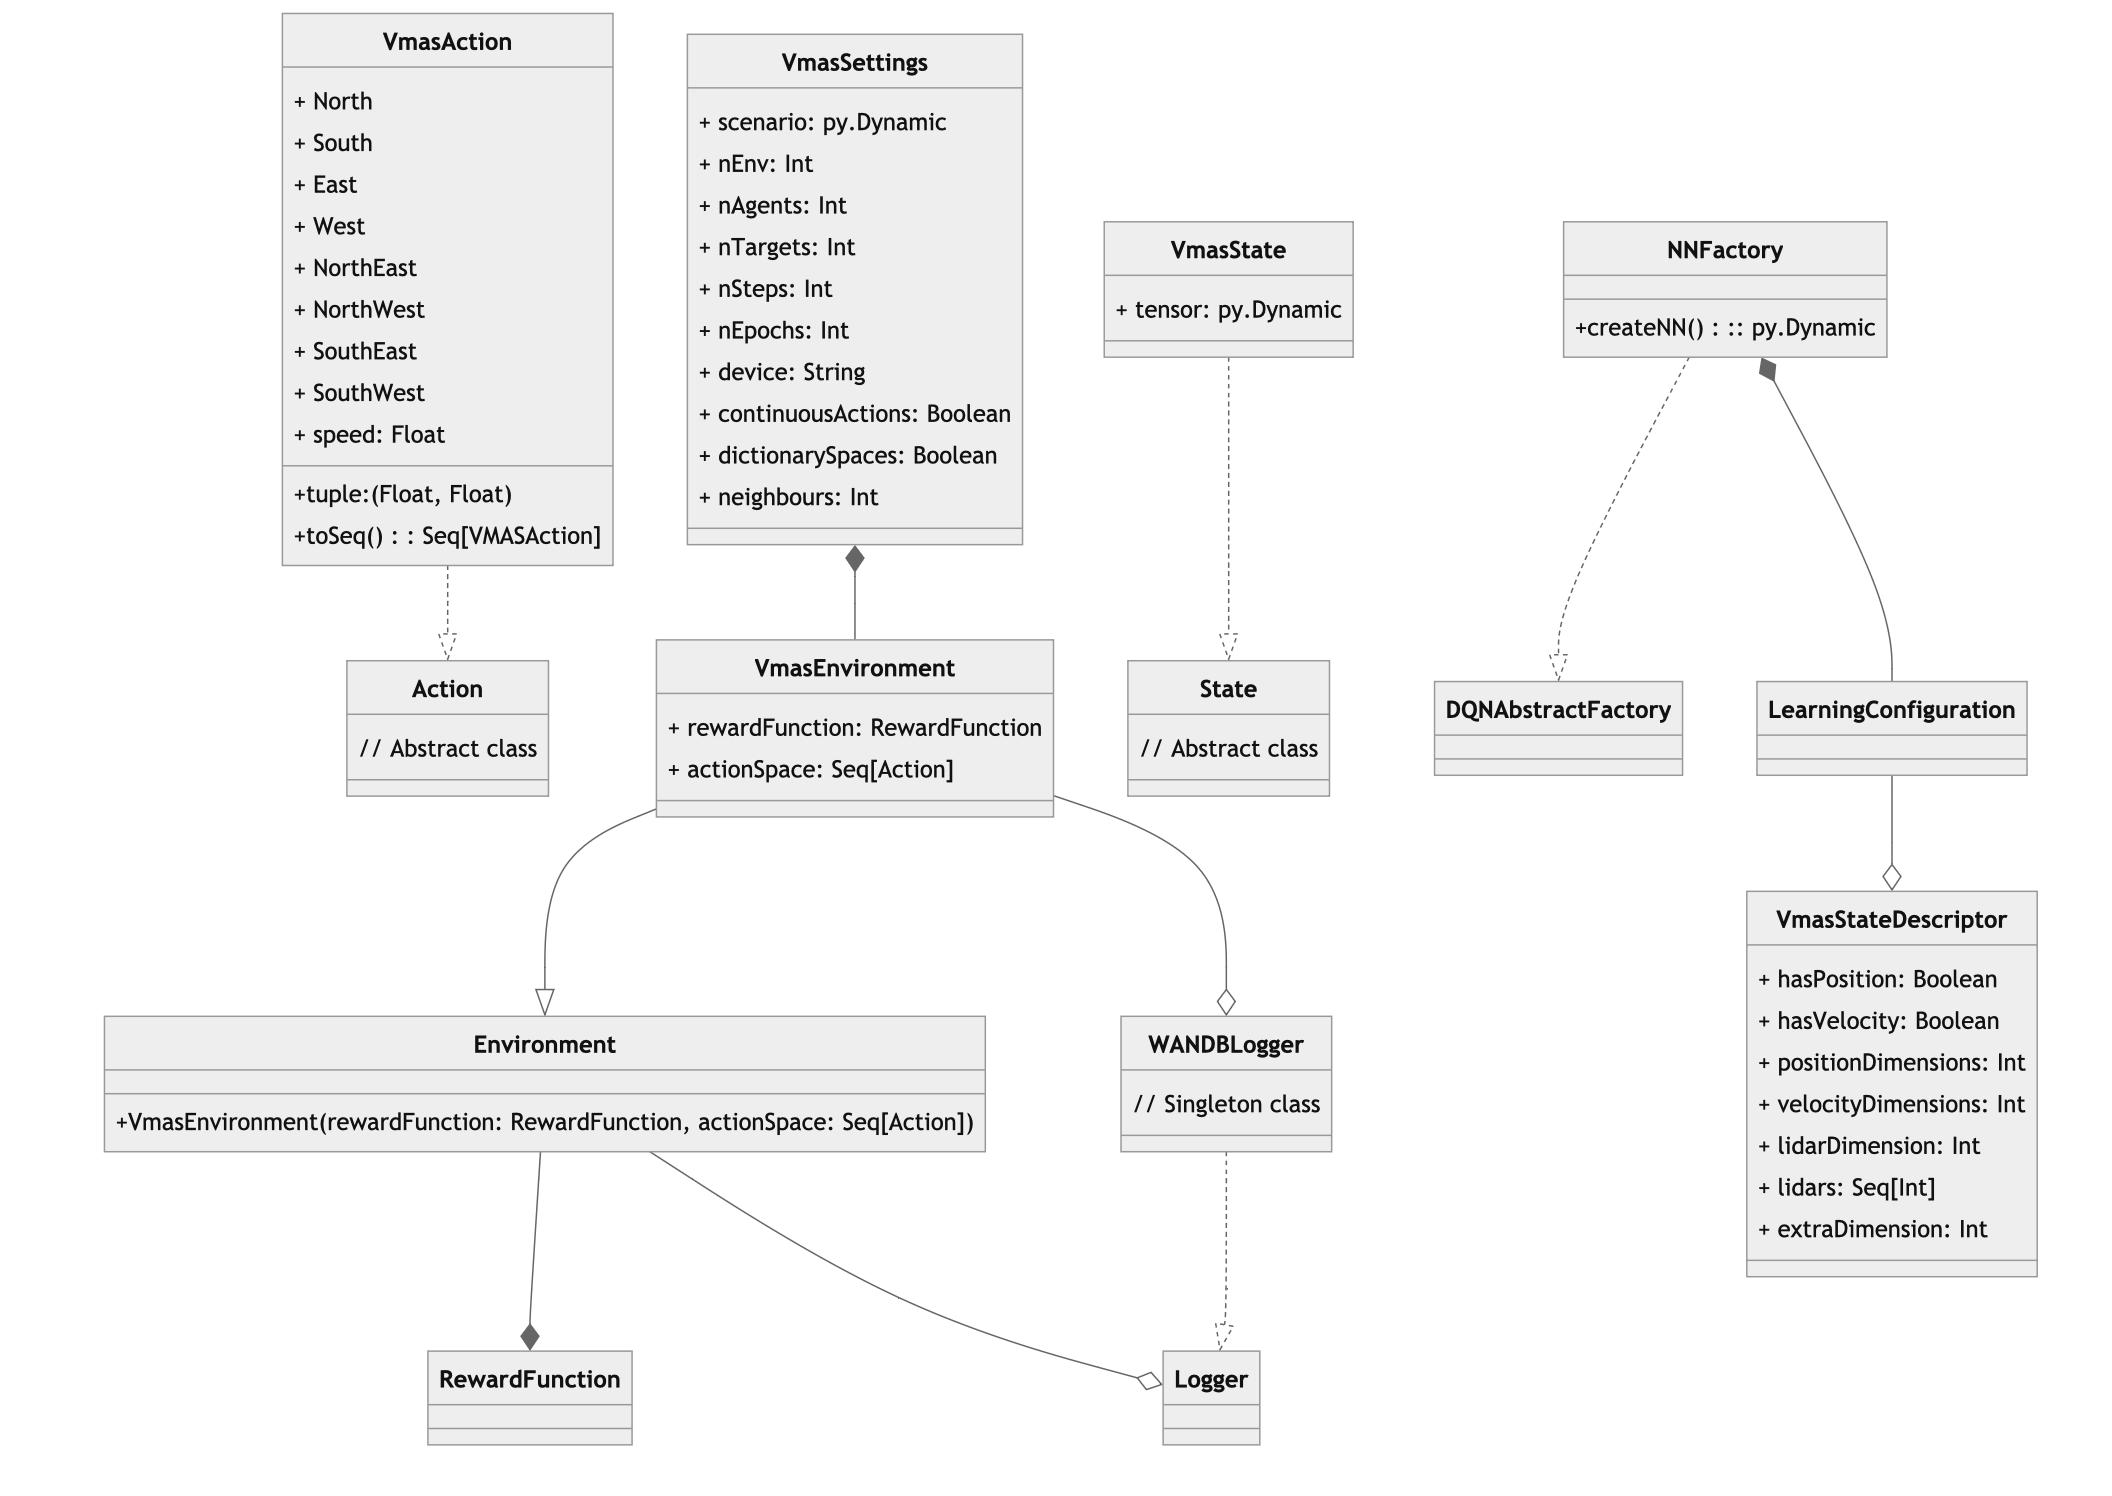
\includegraphics[width=\textwidth]{img/scarlib-vmas.png}
\caption{UML class diagram showing the scarlib-vmas module structure}
\label{fig:scarlib-vmas}
\end{figure}
Being highly flexible and exposing all the necessary interfaces, scarlib seamlessly integrated with \ac{vmas}. The structure remained almost identical, providing ad-hoc implementations of various scarlib-core interfaces (\Cref{fig:scarlib-vmas}), yet remaining generic enough to allow for potential customizations. In addition to the primary implementations, several utility classes were defined to more conveniently encapsulate all the configuration parameters of a complex simulator like \ac{vmas}.
For the sake of interoperability between Scala (and thus Scarlib) and Python (\ac{vmas}), it was not feasible to hide some low-level components behind interfaces, especially the definition of the reward function and the retrieval of observations. In this regard, an implementation of the \ac{vmas} Scenario class must be defined in Python, added to the Python libraries, and then specified by name during the System configuration; an alternative is to provide two lambda functions, one for the reward function and one for the observation, to be used via the strategy pattern in the AbstractScenario python class. 
Luckily, for not complex functions it is also possible to use a dedicated Scala DSL which will then compile to Python code.

\subsection{Actions and states}
By default the \emph{scarlib-vmas} module offers an implementation of both the state and actions interfaces; more specifically, up to eight actions are already defined, allowing for movements in a bidimensional space in the four cardinal directions and the four ordinal (or intercardinal) directions.
Moreover, a companion object is also present to easily map the actions to their respective \emph{PyTorch} tensor, masking the underlying complexion.
Reguarding the states, instead, a wrapper has been implemented to easily manage the attached tensors, without having to perform complicated math to define their shapes; in fact, an utility class called \emph{VmasStateDescriptor} allows you to retrieve the final shape of a tensor based on the configuration parameters, such has number and size of \emph{LiDARs}, if the environment is keeping track of agents position and velocity, and eventual extra dimensions (e.g. positions of neighbours).

\begin{lstlisting}
    case class VmasStateDescriptor(hasPosition: Boolean = true, hasVelocity: Boolean = true, 
        positionDimensions: Int = 2, velocityDimensions: Int = 2, lidarDimension: Int = 1, 
        lidars: Seq[Int] = Seq.empty, extraDimension: Int = 0) {
    def getSize: Int = {
        var totalSize = extraDimension
        if (hasPosition) totalSize += positionDimensions
        if (hasVelocity) totalSize += velocityDimensions
        if (lidars.nonEmpty) totalSize += lidars.sum * lidarDimension
        return totalSize
    }
}
\end{lstlisting}

For example, to define a state which keeps track of the agent position and of the the closest \emph{nNeighbour} positions 
the following setup could be used:
\begin{lstlisting}
    val stateDescriptor = VmasStateDescriptor(hasPosition=true, hasVelocity=false, 
        extraDimension = nNeighbour * 2)
    VMASState.setDescriptor(stateDescriptor)
    val factory = new NNFactory(stateDescriptor, VMASAction.toSeq)
\end{lstlisting}

\subsection{Environment}
The environment customizations specific for \ac{vmas} have been implemented in the \emph{VmasEnvironment} class that extends the \emph{Environment} class of ScaRLib core.
To make it compatible with the DSL and to also simplify its configuration, the constructor has been kept identical to the parent class, grouping all the possible
settings in a class called \emph{VmasSettings}.
\begin{lstlisting}
    case class VmasSettings(
                         scenario: py.Dynamic,
                         nEnv: Int = 1,
                         nAgents: Int = 1,
                         nTargets: Int = 0,
                         nSteps: Int = 1000,
                         nEpochs: Int = 1,
                         device: String = AutodiffDevice().as[String],
                         continuousActions: Boolean = true,
                         dictionarySpaces: Boolean = true,
                         neighbours: Int = 0
                       )
\end{lstlisting}
The most important parameter to configure is the scenario: defined as an instance of \emph{py.Dynamic} (a \emph{ScalaPy} trait that masks a dynamic Python object),
it represents the Python class containg the scenario definition.
\begin{lstlisting}
    val scenario = py.module("CohesionAndCollisionNoLidar").Scenario()
\end{lstlisting}
The biggest constraint is that the module name, in the example \emph{CohesionAndCollisionNoLidar}, has to be included in the \emph{Python PATH}, either by local or global environment variable.
The other parameters of the \emph{VmasSettings} class are pretty straightforward:
\begin{enumerate}
    \item \emph{nEnv}: the number of parallel environments
    \item \emph{nAgents}: the number of total agents
    \item \emph{nTargets}: the number of total targets
    \item \emph{nSteps}: the number of steps for each epoch
    \item \emph{nEpochs}: the number of epochs for the training or validation
    \item \emph{device}: the device on which the tensors are stored, either CPU (\emph{cpu}) or GPU (\emph{cuda})
    \item \emph{continuousActions}: flag to enable floating points for the agents positions
    \item \emph{dictionarySpaces}: flag to decide if \ac{vmas} should return the observations and the rewards as dictionaries with key the agents ids
    \item \emph{neighbours}: the number of neighbours each agent will be looking for
\end{enumerate}

Given the tensor-based architecture of \ac{vmas}, a step of an environment consist in executing all the actions of the agents at the same time; that introduces 
a compatilibity issue with ScaRLib which performs the agent's action sequentiallly.
\begin{lstlisting}
override def step(action: Action, agentId: Int): Future[(Double, State)] = {
        actions = actions :+ action.asInstanceOf[VMASAction].toTensor()
        val nAgents: Int = env.n_agents.as[Int]
        val isLast = nAgents - 1 == agentId
        val promise = scala.concurrent.Promise[(Double, State)]()
        val future = promise.future
        promises = promises :+ promise
        if (isLast) {
            steps += 1
            val result = env.step(actions.toPythonCopy)
            actions = Seq[py.Dynamic]()
            val observations = result.bracketAccess(0)
            val rewards = result.bracketAccess(1)
            for (i <- 0 until nAgents) {
                val agentName = "agent_" + i
                val reward = rewards.bracketAccess(agentName).as[Double]
                AgentGlobalStore().put(i, s"agent-$i-reward", reward)
                val observation = observations.bracketAccess(agentName)
                val state = new VMASState(observation)
                lastObservation = lastObservation.updated(agentId, Some(state))
                promises(i).success((reward, state))
            }
            promises = Seq[scala.concurrent.Promise[(Double, State)]]()
        }
        return future
    }
\end{lstlisting}
In order to make it work, each agent is iterated over and associated to a promise; when the last agent is reached, all the agents actions are performed and then the promises are resolved iterating over each agent reward.

\subsection{Rendering}
\ac{vmas} offers an out of the box renderer based on \emph{OpenGL}, which means that in order to use an \emph{OpenGL enabled GPU} is in order.
The rendering, unfortunately, is still unoptimized, requiring a lot of time to process a single frame; the lack of optimization is especially evident when the number of agents is in the order of hundreds, requiring dozens of minutes if not hours.
To mitigate this issue and avoind the blocking of the simultation thread, all the rendering is performed on a separate thread, generating a promise for each frame; the promises are then joined on an arbitrary thread to generate the final gif image.
It is important to notice that the rendering thread has to be the same because \emph{OpenGL} only support one execution context per instance, thus preventing any attempt at a parallelized approach; even tough a second context might be introduced, it is not feasible since it introduces too much complexity.

\subsection{Logging}

\begin{figure}[t]
    \centering
    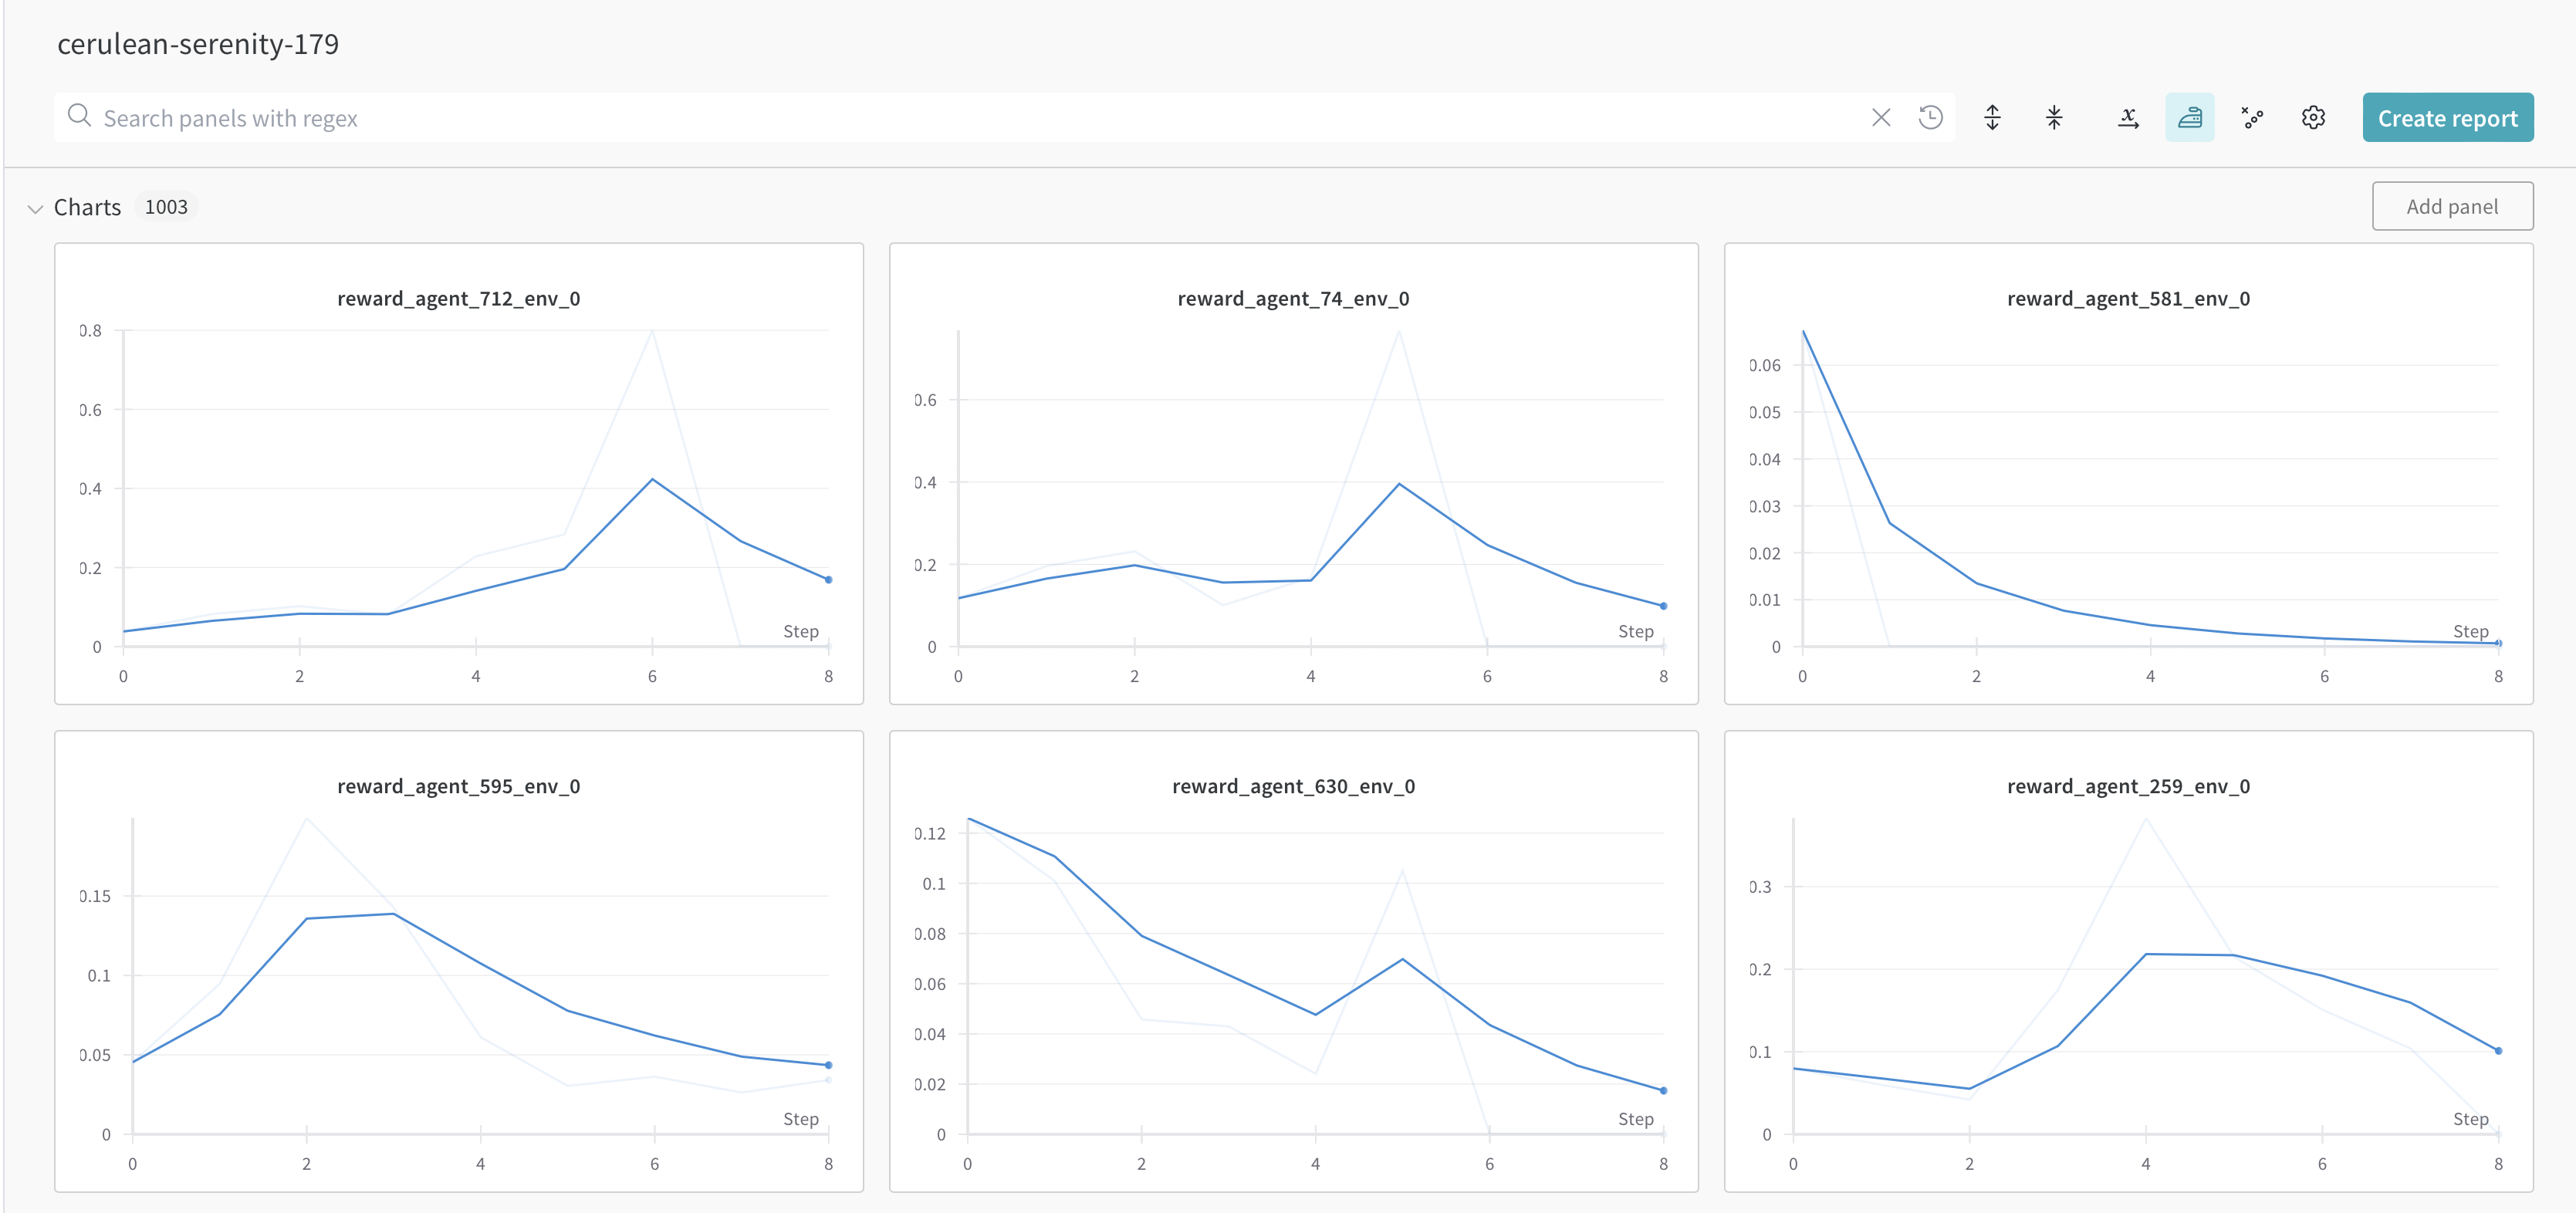
\includegraphics[width=\textwidth]{img/wandb.png}
    \caption{Dashboard with the results of a simulation}
    \label{fig:wandb}
\end{figure}

As an alternative to \emph{TensorBoard}, the \emph{scarlib-vmas} module introduces the \emph{WANDBLogger} class, a facade to use the ScaRLib logging APIs while saving the logs on WANDB's cloud (\Cref{fig:wandb}).

\subsection{Reward and observation functions}
There are three possible way to define the reward and observation functions. The first one consist in defining them in the \emph{Scenario} implementation in Python, as was done with the \emph{CohesionAndCollisionNoLidar} example; this approach, even if it works, forces the user to edit multiple times the environment variables to add all the \emph{Scenari} classes to the \emph{Python PATH}, making it prone to errors and time consuming.\\
\begin{lstlisting}[language=scala]
    val scenario = py.module("CohesionAndCollisionNoLidar").Scenario()
\end{lstlisting}
The second approach is more versatile, as it works using two \emph{lambda} and then by providing them to the \emph{AbstractScenario} class during instantiation; this way the \emph{Python PATH} as to be configured once and via the strategy pattern it can be customized on demand.
\begin{lstlisting}[language=scala]
    CPythonInterpreter.execManyLines(
        """def rf(env, agent):
            import torch
            import math
            agents = agent.obs
            
            [...] #factors calculations

            result = cohesion_factor + collision_factor
            return torch.tensor(result, device=env.world.device).squeeze(0)
          """
    )
    val rfLambda = py.Dynamic.global.rf
    CPythonInterpreter.execManyLines(
        """def obs(env, agent):
            import torch
            
            [...] #observations calculation

            result = torch.cat([agent_pos_to_device.squeeze(0), agent.obs.view(10)], dim=-1)
            return result.unsqueeze(0)
    """)
    val obsLambda = py.Dynamic.global.obs
    val scenario = py.module("AbstractEnv").Scenario(rfLambda, obsLambda)
\end{lstlisting}

In case of reward functions that do not require complex logic, the vmas module provides a DSL to easily define a reward function and then translate to Python code.
\begin{lstlisting}[language=scala]
    val rf = AddRoot(10.0, CurrentState) ++ AddRoot(-5.5, NewState) + Tensor(5) --> Lambda("x: x") >> Lambda("x: x.min()")
    val obsLambda = py.Dynamic.global.obs
    //By calling toString() on the result of the DSL operations you will get the equivalent Python code to be provided as a lambda to the scenario
    val scenario = py.module("AbstractEnv").Scenario(rf.toString(), obsLambda)
\end{lstlisting}
A much more detailed explanation of the DSL capabilities will be found in the next chapter.
\subsection{DSL}
This integration is of course compatible with the DSL already offered by ScaRLib. Apart from a few configuration classes, the remaing components of the simulator can be 
easily instantiated using the DSL:
\begin{lstlisting}
    WANDBLogger.init()
    private val nNeighbour = 5
    val stateDescriptor = VmasStateDescriptor(hasPosition=true, hasVelocity=false, 
        extraDimension = nNeighbour * 2)
    VMASState.setDescriptor(stateDescriptor)
    val scenario = py.module("CohesionAndCollisionNoLidar").Scenario()
    private val envSettings = VmasSettings(scenario = scenario, nEnv = 1, nAgents = nAgents, 
        nTargets = 0,nSteps = nSteps, nEpochs = 150, device = "cpu", 
        neighbours = nNeighbour)
    implicit val configuration: Environment => Unit = (e: Environment) => {
        val env = e.asInstanceOf[VmasEnvironment]
        env.setSettings(envSettings)
        env.setLogger(WANDBLogger)
        env.enableRender(false)
    }
    private val where = s"./networks"
    val system = CTDELearningSystem {
        rewardFunction { null }
        actionSpace { VMASAction.toSeq }
        dataset { ReplayBuffer[State, Action](10000) }
        agents { 200 }
        learningConfiguration {
            LearningConfiguration(dqnFactory = 
                new NNFactory(stateDescriptor, VMASAction.toSeq), snapshotPath = where)
        }
    }(ExecutionContext.global, VMASState.encoding)
    system.learn(envSettings.nEpochs, envSettings.nSteps)
\end{lstlisting}

As anticipated in the previous chapter, another DSL has been provided to facilitate the definition of reward functions. By leveraging implicitic conversions and extensions methods, it was possible to create a simple algebra that supports the following operations:
\begin{enumerate}
    \item \textbf{Root operations:} 
          a root is a starting point for the calculations of the reward function, 
          it can either be the current state or the new state and can be specified 
          using the enum \lstinline{RewardFunctionStepParam.<CurrentState/NewState>}. 
          Four basic operations are supported when defining roots:
          \begin{enumerate}
              \item \lstinline{AddRoot(Any, RewardFunctionStepParam)}: 
                    adds a \textbf{scalar} or \textbf{Tensor} to the specified state. \\
                    Eg: \lstinline{AddRoot(Tensor(5.0), NewState)}
              \item \lstinline{SubRoot(Any, RewardFunctionStepParam)}: 
                    subtracts a \textbf{scalar} or \textbf{Tensor} from the specified state. \\
                    Eg: \lstinline{AddRoot(-10, CurrentState)}
              \item \lstinline{MulRoot(Any, RewardFunctionStepParam)}: 
                    multiplies the specified state by a \textbf{scalar} or \textbf{Tensor}. \\
                    Eg: \lstinline{MulRoot(Tensor(-5.0), NewState)}
              \item \lstinline{DivRoot(Ant, RewardFunctionStepParam)}: 
                    divides the specified state by a \textbf{scalar} or \textbf{Tensor}. \\
                    Eg: \lstinline{DivRoot(17.56, CurrentState)}
          \end{enumerate}
          
    \item \textbf{Roots fusion operations:} 
          operations between two root nodes are performed using special operators:
          \begin{enumerate}
              \item \textbf{++}: 
                    it sums the values of the two nodes. \\
                    Eg. \lstinline|AddRoot(Tensor(5.0), NewState) ++ MulRoot(Tensor(-5.0), CurrentState)|
              \item \textbf{--}: 
                    it subtracts the value of the second node from the first one. \\
                    Eg. \lstinline|AddRoot(Tensor(5.0), NewState) -- AddRoot(Tensor(-10.0), NewState)|
              \item \textbf{**}: 
                    it multiplies the values of the two nodes. \\
                    Eg. \lstinline|AddRoot(Tensor(5.0), NewState) ** MulRoot(Tensor(-5.0), CurrentState)| 
              \item \textbf{\textbackslash\textbackslash}: 
                    it divides the value of the first node by the value of the second one. \\
                    Eg. \lstinline[language=scala]|AddRoot(Tensor(5.0), NewState) \\ AddRoot(Tensor(-10.0), NewState)| 
          \end{enumerate}
          
    \item \textbf{Scalar and tensor operations:}
          \begin{enumerate}
              \item \textbf{+} : 
                    it sums a \textbf{scalar} or \textbf{Tensor} to another node, \\
                    either a \textbf{scalar} or \textbf{Tensor} or root node. \\
                    Eg. \lstinline|Tensor(10) + 5|
              \item \textbf{-} : 
                    it subtracts a \textbf{scalar} or \textbf{Tensor} from another node, \\
                    either a \textbf{scalar} or \textbf{Tensor} or root node. \\
                    Eg. \lstinline|AddRoot(2, CurrentState) - 10|
              \item \textbf{*} : 
                    it multiplies another node, 
                    either a \textbf{scalar} or \textbf{Tensor} or root node, \\
                    by a \textbf{scalar} or \textbf{Tensor}. \\
                    Eg. \lstinline|Tensor(20) - Tensor(3)|
              \item \textbf{/} : 
                    it divides another node, \\
                    either a \textbf{scalar} or \textbf{Tensor} or root node, \\
                    by a \textbf{scalar} or \textbf{Tensor}. \\
                    Eg. \lstinline|SubRoot(1, NewState) / Tensor(2.5)|
          \end{enumerate}
          
    \item \textbf{Map operation ($->$):} 
          the map operation allows mapping each value of a node to another value using a \emph{lambda}; 
          the \emph{lambda} is created using the \lstinline|Lambda(String)| class, 
          where the string parameter is the Python code containing the logic. 
          Eg. \lstinline|AddRoot(0, CurrentState) -> Lambda("x: math.sqrt(Float(x))")|
          
    \item \textbf{Reduce operation ($>>$):} 
          the reduce operation transforms the value of a node to a double; 
          as with the map operation, it accepts a \emph{lambda}, 
          but a type check on the returned value is performed to be sure 
          that the final value is indeed a double; 
          Eg. \lstinline|AddRoot(0, CurrentState) >> Lambda("x: x.min()[0]")|
\end{enumerate}


\chapter{Validation} % possible chapter for Projects
\label{chap:validation}

\section{Cohesion and Collision performance comparison with Alchemist}
\subsection{Implementation}
\ac{vmas} does not offer a neighbouring system as \emph{Alchemist} does, which means that a custom solution has to be implented. 
A trivial approach would be to use the \emph{LiDAR} sensors to detect the \emph{closest N detected agents}; unfortunately, while this approach theoretically works, it is not feasible when working with hundreds of agents due to the computational complexity.
The best solution is to calculate a matrix wich has as row and column indices the agents ids, and the value of its cells the distances between those agents; while it might seem as complex as the \emph{LiDAR} approach, there are a few \emph{PyTorch} functions designed to do this using state of the art algorithms.
\begin{lstlisting}
    agents_positions = torch.stack([t.state.pos for t in self.world.agents], dim=1).squeeze(0).to(self.world.device)
    distances = torch.cdist(agents_positions, agents_positions)
    # Exclude the agent itself by setting diagonal elements to a large value
    distances.fill_diagonal_(float('inf'))
    # Sort distances along the second dimension (axis 1)
    sorted_distances, indices = torch.sort(distances, dim=1)
    # Select the top 5 indices for each agent
    self.distances = sorted_distances[:, :5]
    self.top_indices = indices[:, :5]
    self.top_positions = agents_positions[self.top_indices, :]
\end{lstlisting}
Once the position of the neighbours has been retrieved, the calculation for the agent reward is pretty streighforward:
\begin{lstlisting}
    def cohesionFactor(self, distances):
        max_distance = distances[4]
        return -(max_distance - self.target_distance) if max_distance > self.target_distance else 0.0

    def collisionFactor(self, distances):
        min_distance = distances[0]
        if min_distance == 0: return -100
        return 0 if min_distance >= self.target_distance else 2 * math.log(min_distance / self.target_distance)
    
    def reward(self, agent):
        agents = agent.obs
        if agents is None:
            return torch.zeros(self.world.batch_dim, dtype=torch.float32, device=self.world.device)
        agent_id = int(agent.name.split("_")[1])
        distances = self.distances[agent_id]

        cohesion_factor = self.cohesionFactor(distances)
        collision_factor = self.collisionFactor(distances)
        result = cohesion_factor + collision_factor
        return tensor(result, device=self.world.device).squeeze(0)
\end{lstlisting}
\subsection{Results comparison}
The \emph{Cohesion and Collision} scenario has been simulated on both \ac{vmas} and Alchemist using different amounts of agents: 200, 1000, 5000 and 10000 (\Cref{tab:comparison}).\\
While both \ac{vmas} and Alchemist were able to execute the simulations with 200 and 1000 agents, only \ac{vmas}, given enough time, managed to complete the simulations with 5000 and 10000 agents.
\begin{table}
    \caption{Performance comparison for the scenario Cohesion and Collision using Alchemist and VMAS with different amounts of agents}
\begin{center}
    \begin{tabular}{ |c|c|c| } 
     \hline
     Agents & \ac{vmas} & Alchemist \\ 
     200 & 2 minutes & 1 minutes \\ 
     1000 & 30 minutes & 16 minutes \\ 
     5000 & 7 hours & $\infty$ \\ 
     10000 & 15 hours & $\infty$ \\ 
     \hline
    \end{tabular}
    \label{tab:comparison}
\end{center}
\end{table}
\begin{figure}[t]
    \centering
    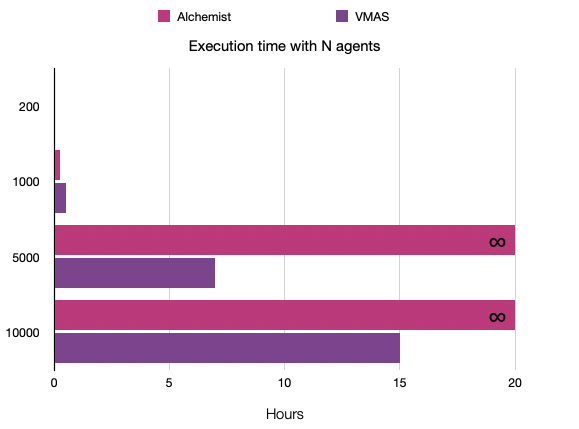
\includegraphics[width=\textwidth]{img/cohandcoll-vmas-alchemist.png}
    \caption{\ac{vmas} and Alchemist performances on different configurations of the Cohesion and Collision scenario}
    \label{fig:cohandcoll-vmas-alchemist}
\end{figure}
It appears that with a reduced number of agents, Alchemist outperforms \ac{vmas} by an average of 50\% less time to complete the simulation; on the contrary, when the number of agents start to increase past the thousand, Alchemist is no longer able to execute the simulation, sometimes not even starting at all, while \ac{vmas}, even tough in many hours, can do so.
The figure (\Cref{fig:cohandcoll-vmas-alchemist}) illustrates how impactful can the use of \ac{vmas} be when working with \ac{marl} systems.

\section{Usage showcase: Cleaning Agents scenario}

The \emph{Cleaning Agents} scenario within \ac{vmas} presents a challengin \ac{marl} environment. In this scenario, a team of \emph{N agents} is tasked with cleaning a 2D space by removing \emph{M stationary targets}. This scenario might serve as a valuable benchmark for evaluating the coordination and decision-making capabilities of \ac{marl} algorithms executed on the \emph{scarlib-vmas} module.

\subsection{Agents and Sensors}

Each agent in the \emph{Cleaning Agents} scenario is equipped with a specialized \emph{LiDAR} sensor that projects 50 rays into the environment.
This sensor is designed to detect only targets within its range.
The purpose of the \emph{LiDAR} sensor is to enable agents to perceive the presence and location of targets, crucial for their cleaning task.

\subsection{Objective}

The primary goal of the agents in this scenario is to efficiently remove all \emph{M targets} from the 2D space. To successfully remove a target, an agent must be in close proximity to it, ensuring effective cleaning. This proximity requirement adds complexity to the task, as agents must navigate and coordinate to reach and clean targets efficiently.

\subsection{Reward Function}

The reward function in the \emph{Cleaning Agents} scenario is designed to encourage agents to make optimal decisions while cleaning the targets. The reward function operates as follows:
\begin{enumerate}
  \item When an agent's distance from a target falls below a predefined threshold (K), indicating successful cleaning, the agent is rewarded positively:
  \emph{Reward = $1 + \text{number of previously removed targets}$}
  \item If an agent's \emph{LiDAR} sensor does not detect any targets in its vicinity, it receives a negative reward (-1):
  \emph{Reward = $-1$}
  \item When an agent's \emph{LiDAR} sensor detects a target, and the distance from the agent's previous position to the target decreases, the agent is rewarded based on the function:
  \emph{Reward = }$\frac{-\text{LIDAR range}}{x}$ \emph{(normalized to fall within the range of -0.5 to 0)}
  \item Conversely, if the distance from the agent's previous position to the target increases, indicating a suboptimal move, the agent is penalized based on the same function:
  \emph{Reward = }$\frac{-\text{LIDAR range}}{x}$ \emph{(normalized to fall within the range of -1 to -0.5)}
\end{enumerate}
The strategic use of negative rewards, except for successful target removal, ensures that agents are motivated to make coordinated and efficient moves. It encourages agents to continually improve their performance by minimizing suboptimal actions and maximizing successful cleaning operations.

The \emph{Cleaning Agents} scenario in \ac{vmas} thus presents a dynamic and challenging environment that tests the coordination, navigation, and decision-making capabilities of \ac{marl} algorithms in the context of multi-agent systems.

\subsection{Implementation}

\subsubsection{Deep Q Learning for MLP Networks}

The implementation of DQL for \emph{Multilayer Perceptron (MLP)} networks is designed to accommodate the unique 
characteristics of the \acf{vmas} environment. It employs additional dimensions to parallelize 
environments and agents, necessitating a flexible approach to handle complex tensor shapes.

\paragraph{State Representation}

In such implementation, it is employed a state representation that aligns with the structure of \ac{vmas}. Specifically, the state of each agent is represented as a tensor of shape [50, 1]. This choice is informed by the fact that each agent's \emph{LiDAR} sensor in \ac{vmas} emits 50 rays, returning float distances. The positions of the individual agents within the environment are not considered relevant for decision-making since agents rely solely on \emph{LiDAR} measurements, and the positions of targets can vary across different \ac{vmas} environments.

\paragraph{Tensor Shapes}

To facilitate the training and execution of the MLP networks within \ac{vmas}, the network architecture accommodates tensors with the shape [number of environments, number of agents, 50, 1]. This tensor shape aligns with \ac{vmas}'s parallelized structure, allowing the network to process data from multiple environments and agents simultaneously.

By adapting the DQL implementation to handle tensors of complex shapes, a seamless integration with \ac{vmas}'s multi-agent framework is ensured. This flexibility enables agents to effectively learn and make decisions within the dynamic and parallelized \ac{vmas} environment, ultimately enhancing their performance in complex multi-agent tasks.

\newpage

\subsection{Results}
\subsubsection{Performance Results: MLP Networks in the Cleaning Agents Scenario}

The performance evaluation of the MLP network-based agents in the \emph{Cleaning Agents} scenario provides valuable insights into their learning and decision-making capabilities. The training process consisted of \emph{150 epochs, each comprising 1000 steps}. If an agent successfully achieved its task before completing all the steps in an epoch, it proceeded to the next epoch. Here it is presentent a comprehensive analysis of the training and evaluation results.

\paragraph{Training Progress}

\begin{figure}
  \centering
  \begin{subfigure}[b]{0.45\textwidth}
      \centering
      \includegraphics[width=\textwidth]{img/rewards_50_epochs.png}
      \caption{Total reward after 50 epochs}
      \label{fig:g}
  \end{subfigure}
  \hfill
  \begin{subfigure}[b]{0.45\textwidth}
      \centering
      \includegraphics[width=\textwidth]{img/loss_50_epochs.png}
      \caption{Total loss after 50 epochs}
      \label{fig:h}
  \end{subfigure}
  \hfill
  \begin{subfigure}[b]{0.45\textwidth}
      \centering
      \includegraphics[width=\textwidth]{img/rewards.png}
      \caption{Total reward after 150 epochs} 
      \label{fig:i}
  \end{subfigure}
  \hfill
  \begin{subfigure}[b]{0.45\textwidth}
      \centering
      \includegraphics[width=\textwidth]{img/loss.png}
      \caption{Total loss after 150 epochs} 
      \label{fig:l}
  \end{subfigure}
  \caption{Reward and Loss comparison}
  \label{fig:s}
\end{figure}

During the initial epoch, agents exhibited limited familiarity with the task of removing targets from the 2D environment. Consequently, the mean reward achieved by the agents in this phase remained relatively low, with a maximum reward of approximately \emph{3.0}. As training progressed, agents displayed improved performance (\Cref{fig:g}). By the \emph{70th epoch}, the highest recorded mean reward reached \emph{8.0}, typically occurring at around \emph{900 steps} into the episode. This milestone indicated that agents had grasped the fundamentals of their task but still had room for refinement.

A significant leap in performance was observed at the \emph{145th epoch} (\Cref{fig:i}). Agents demonstrated remarkable efficiency by removing almost all targets \emph{in fewer than 500 steps}, with the last remaining target eliminated in the final steps of the episode. Concurrently, the loss function exhibited a notable pattern. While initially showing spikes when agents were rewarded values exceeding \emph{1.0} (\Cref{fig:h}), the loss gradually minimized and stabilized \emph{near zero} after the \emph{100th epoch} (\Cref{fig:l}).

\begin{figure}
  \centering
  \begin{subfigure}[b]{0.45\textwidth}
      \centering
      \includegraphics[width=\textwidth]{img/mean_reward_1_epoch.png}
      \caption{Mean Reward Epoch 1}
      \label{fig:d}
  \end{subfigure}
  \hfill
  \begin{subfigure}[b]{0.45\textwidth}
      \centering
      \includegraphics[width=\textwidth]{img/mean_reward_70_epoch.png}
      \caption{Mean Reward Epoch 70}
      \label{fig:e}
  \end{subfigure}
  \hfill
  \begin{subfigure}[b]{0.45\textwidth}
      \centering
      \includegraphics[width=\textwidth]{img/mean_reward_145_epoch.png}
      \caption{Mean Reward Epoch 145} 
      \label{fig:f}
  \end{subfigure}
  \caption{Mean rewards}
\end{figure}

\paragraph{Evaluation Results}

\begin{figure}
  \centering
  \begin{subfigure}[b]{0.45\textwidth}
      \centering
      \includegraphics[width=\textwidth]{img/1_agent_1.png}
      \caption{Beginning of simulation}
  \end{subfigure}
  \hfill
  \begin{subfigure}[b]{0.45\textwidth}
      \centering
      \includegraphics[width=\textwidth]{img/1_agent_2.png}
      \caption{Half simulation}
  \end{subfigure}
  \hfill
  \begin{subfigure}[b]{0.45\textwidth}
      \centering
      \includegraphics[width=\textwidth]{img/1_agent_3.png}
      \caption{End of simulation} 
  \end{subfigure}
  \caption{Different stages of a simulation with one agent and 8 targets}
  \label{fig:m}
\end{figure}

To assess the agents' performance in practical scenarios, I conducted evaluations with varying numbers of agents and targets. In a scenario involving one agent and eight targets (\Cref{fig:m}), the results indicated the following:
\begin{itemize}
  \item \emph{on average}, it took approximately \emph{10 steps} for the agent to remove the first target, reflecting a quick initiation of the cleaning process (\Cref{fig:d});
  \item removal of half the targets occurred, \emph{on average}, in approximately \emph{170 steps}, demonstrating consistent progress (\Cref{fig:e});
  \item to remove all eight targets, agents required \emph{an average of around 1440 steps}, highlighting the complexity of clearing the entire environment (\Cref{fig:f}).
\end{itemize}

\begin{figure}
  \centering
  \begin{subfigure}[b]{0.45\textwidth}
      \centering
      \includegraphics[width=\textwidth]{img/4_agents_1.png}
      \caption{Beginning of simulation}
  \end{subfigure}
  \hfill
  \begin{subfigure}[b]{0.45\textwidth}
      \centering
      \includegraphics[width=\textwidth]{img/4_agents_2.png}
      \caption{Half simulation}
  \end{subfigure}
  \hfill
  \begin{subfigure}[b]{0.45\textwidth}
      \centering
      \includegraphics[width=\textwidth]{img/4_agents_3.png}
      \caption{End of simulation} 
  \end{subfigure}
  \caption{Different stages of a simulation with four agent and 14 targets}
  \label{fig:n}
\end{figure}

In a more challenging scenario with four agents and fourteen targets (\Cref{fig:n}), the outcomes were as follows:
\begin{itemize}
  \item agents demonstrated improved collaboration, taking \emph{an average of about 400 steps} to clear all fourteen targets;
  \item the first target was removed in \emph{an average of 10 steps}, emphasizing swift task initiation;
  \item removal of half the targets was achieved in \emph{approximately 240 steps}, showcasing efficient teamwork among agents.
\end{itemize}

\begin{figure}
\includegraphics[width=\textwidth]{img/active-targets-per-step.png}
\caption{Remaining targets at each step}
\label{fig:o}
\end{figure}

These performance results underscore the adaptability and learning capabilities of the MLP network-based agents in the \emph{Cleaning Agents} scenario. As training progressed, agents demonstrated a substantial improvement in their task execution, achieving efficient target removal even in scenarios with multiple agents and numerous targets (\Cref{fig:o}).
These findings reflect the effectiveness of this \ac{rl} approach in addressing complex multi-agent coordination tasks.

\newpage

\chapter{Conclusion}
\label{chap:conclusion}
The importance of Multi-Agent Reinforcement Learning (MARL) systems has been gaining significant momentum. As a result, the call to develop modern frameworks, as well as enhance existing ones, stands heightened. Possessing the distinction of being the only framework for MARL in Scala, ScaRLib asserts its potential for greater usage. However, the inability to conduct massive simulations with numerous agents prevents its adoption on a broader spectrum.

The integration with VMAS emerged as the remedy to this issue. Despite these larger simulations demanding substantial time investments, they offered access to a realm of simulations that had, previosuly, been unreachable. An additional merit weighing in favor of the ScaRLib's integration with VMAS is its compatibility to operate seamlessly with RLib. The adaptability permits ScaRLib's execution across a distributed infrastructure, thereby significantly reducing execution times. This advantage positions ScaRLib as a viable option not only for researchers but also for industrial-grade companies.

While functionalities like the physical simulator for gravity, collisions, and \emph{LiDAR} sensors introduced through VMAS may seem tangential to the core thesis, they could potentially be useful for the design of future simulations. The skill gap posed by the need for Python knowledge for the implementation of VMAS scenarios has also been significantly decreased with the development of the ScaRLib-VMAS DSL.

In conclusion, the use of ScaRLib and VMAS demonstrates the transformative potential of sophisticated simulation tools in the field of MARL systems, by also overcoming significant challenges, such as skill-gap barriers due to missing Python knowledge and limitations on large-scale simulations.

\addcontentsline{toc}{chapter}{Bibliography}
%\bibliographystyle{unsrt}
%\bibliography{bibliografia}
\printbibliography %Prints bibliography

\end{document}
